% arara: pdflatex
% arara: pdflatex
% arara: pdflatex

% options:
% thesis=B bachelor's thesis
% thesis=M master's thesis
% czech thesis in Czech language
% slovak thesis in Slovak language
% english thesis in English language
% hidelinks remove colour boxes around hyperlinks

\documentclass[thesis=M,czech]{FITthesis}[2019/03/06]

\usepackage[utf8]{inputenc} % LaTeX source encoded as UTF-8
\usepackage{float}
\usepackage{subfig}
\usepackage{enumitem}
\usepackage{rotating}

\usepackage{newfloat}
\DeclareFloatingEnvironment[placement={!ht},name=Seznam]{mylist}
% \usepackage{amsmath} %advanced maths
% \usepackage{amssymb} %additional math symbols

\usepackage{dirtree} %directory tree visualisation

% % list of acronyms
% \usepackage[acronym,nonumberlist,toc,numberedsection=autolabel]{glossaries}
% \iflanguage{czech}{\renewcommand*{\acronymname}{Seznam pou{\v z}it{\' y}ch zkratek}}{}
% \makeglossaries

\newcommand{\tg}{\mathop{\mathrm{tg}}} %cesky tangens
\newcommand{\cotg}{\mathop{\mathrm{cotg}}} %cesky cotangens

% % % % % % % % % % % % % % % % % % % % % % % % % % % % % % 
% ODTUD DAL VSE ZMENTE
% % % % % % % % % % % % % % % % % % % % % % % % % % % % % % 

\department{Katedra softwarového inženýrství}
\title{MIDI stage piano}
\authorGN{Petr} %(krestní) jméno (jména) autora
\authorFN{Svoboda} %príjmení autora
\authorWithDegrees{Bc. Petr Svoboda} %jméno autora vcetne soucasných akademických titulu
\author{Petr Svoboda} %jméno autora bez akademických titulu
\supervisor{Ing. Josef Pavlíček, Ph.D.}
\acknowledgements{Doplnte, máte-li komu a za co dekovat. V~opacném prípade úplne odstrante tento príkaz.}
% TODO
\abstractCS{V~nekolika vetách shrnte obsah a prínos této práce v~ceštine. Po prectení abstraktu by se ctenár mel mít ctenár dost informací pro rozhodnutí, zda chce Vaši práci císt.}
\abstractEN{Sem doplnte ekvivalent abstraktu Vaší práce v~anglictine.}
\placeForDeclarationOfAuthenticity{V~Praze}
% TODO
\declarationOfAuthenticityOption{4} %volba Prohlášení (císlo 1-6)
\keywordsCS{VST, MIDI, OSC}
\keywordsEN{VST, MIDI, OSC}
% \website{http://site.example/thesis} %volitelná URL práce, objeví se v tiráži - úplne odstrante, nemáte-li URL práce

\begin{document}

% \newacronym{CVUT}{{\v C}VUT}{{\v C}esk{\' e} vysok{\' e} u{\v c}en{\' i} technick{\' e} v Praze}
% \newacronym{FIT}{FIT}{Fakulta informa{\v c}n{\' i}ch technologi{\' i}}

\begin{introduction}
V hudební branži se můžeme setkat s rozličnými hudebními nástroji. V posledních desetiletích
zaujaly významné místo na trhu elektronické hudební nástroje. Zároveň se s příchodem dostupných a výkonných
výpočetních jednotek začaly objevovat virtuální hudební nástroje\cite{kogan2008brief}.
Jedná se o software, který dokáže generovat zvukovou vlnu v reálném čase na základě kofigurovatelných parametrů a vstupů, jako jsou MIDI data, či zvukový signál.
Lze tak dosáhnout věrné simulace syntezátorů, varhan a dalších mnoha hudebních nástrojů, včetně efektů.
Takové nástroje velmi často implementují některé z dostupných API tak, aby je bylo možné použít v různých prostředích.
Dříve byly hlavní doménou virtuálních nástrojů prostředí pro studiovou produkci hudby\cite{leider2004digital}.
V dnešní době, kdy mobilní zařízení dokáží poskytnout dostatečný výkon, stoupá zájem o využití softwarových hudebních nástrojů
při živých vystoupeních. Cílem práce je navrhnout takové řešení, které by umělci poskytovalo dostatečné možnosti a komfort 
pro efektivní využití virtuálních hudebních nástrojů na pódiu.
	%sem napište úvod Vaší práce
\end{introduction}

\chapter{Analýza}
	\section{Požadavky}
		Z praktických zkušeností lze formulovat následující požadavky na řešení, které bude vyhovovat účelu profesionálního živého vystoupení.
		Jelikož lze požadavky formulovat pouze na obecné úrovni, následuje jejich bodové vyjádření.
		
		Funkční požadavky:
		\begin{itemize}
			\item Ovládací prvky musí být snadno dostupné.
			\item Ovládací prvky musí být precizně ovladatelné.
			\item Uživatel musí být schopen určit aktuální stav systému vizuálním vjemem.
			\item Uživatel může definovat svojí sadu zvuků.
			\item Uživatel může přepínat zvuky z přednastavené sady.
			\item Uživatel může ovládat parametry zvuku v reálném čase.
			\item Uživatel může uložit aktuální zvuk.
			\item Uživatel může ovládat bězné parametry systému, jako např. hlasitost, transpozice.
		\end{itemize}
	
		Nefunkční požadavky:
		\begin{itemize}
			\item Systém nesmí přestat reagovat.
			\item Systém nesmí generovat nežádoucí zvuky.
			\item Systém musí správně ukládat konfiguraci poskytnutou uživatelem.
			\item Systém nesmí umělce omezovat dlouhou dobou prodlevy.
		\end{itemize}
		
	\section{Průzkum existujících řešení}
		\subsection{Hardwarové nástroje}
			Mezi hardwarovými hudebními nástroji se lze setkat s různou mírou optimalizace pro živá vystoupení.
			Zde budeme uvažovat pouze skupinu nástrojů, která je tomuto účelu nejblíže, tzv. stage piana.
			
			Tyto nástroje často poskytují obsáhlou banku zvuků, propracované uživatelské rozhraní a velmi vysokou stabilitu.
			Pokročilejší modely disponují možností přidat nové zvuky v proprietárním formátu, které může uživatel vytvořit za pomocí speciálního nástroje nebo je získat z online databáze. Některé modely navíc umožňují připojit další klaviaturu přes MIDI rozhraní, to ovšem přináší jistá omezení,
			například absenci možnosti použít zvuk stejného typu na obou klaviaturách současně, jelikož zařízení disponuje pouze jedním zvukovým modulem
			pro daný typ zvuku.
			Zároveň nástroje poskytují bohaté možnosti nastavení běžných parametrů, jako jsou např. hlasitost, transpozice, rozdělení klaviatury do zón,
			citlivost klaviatury apod.
			
			Typickým zástupcem jsou modely značky Nord (obr. \ref{fig:HardwareStagepiano}), které jsou velmi oblíbené pro svoji stabilitu a mnohostrannost, jsou nicméně poměrně nákladnou záležitostí.
			
			\begin{figure}[H]
				\centering
				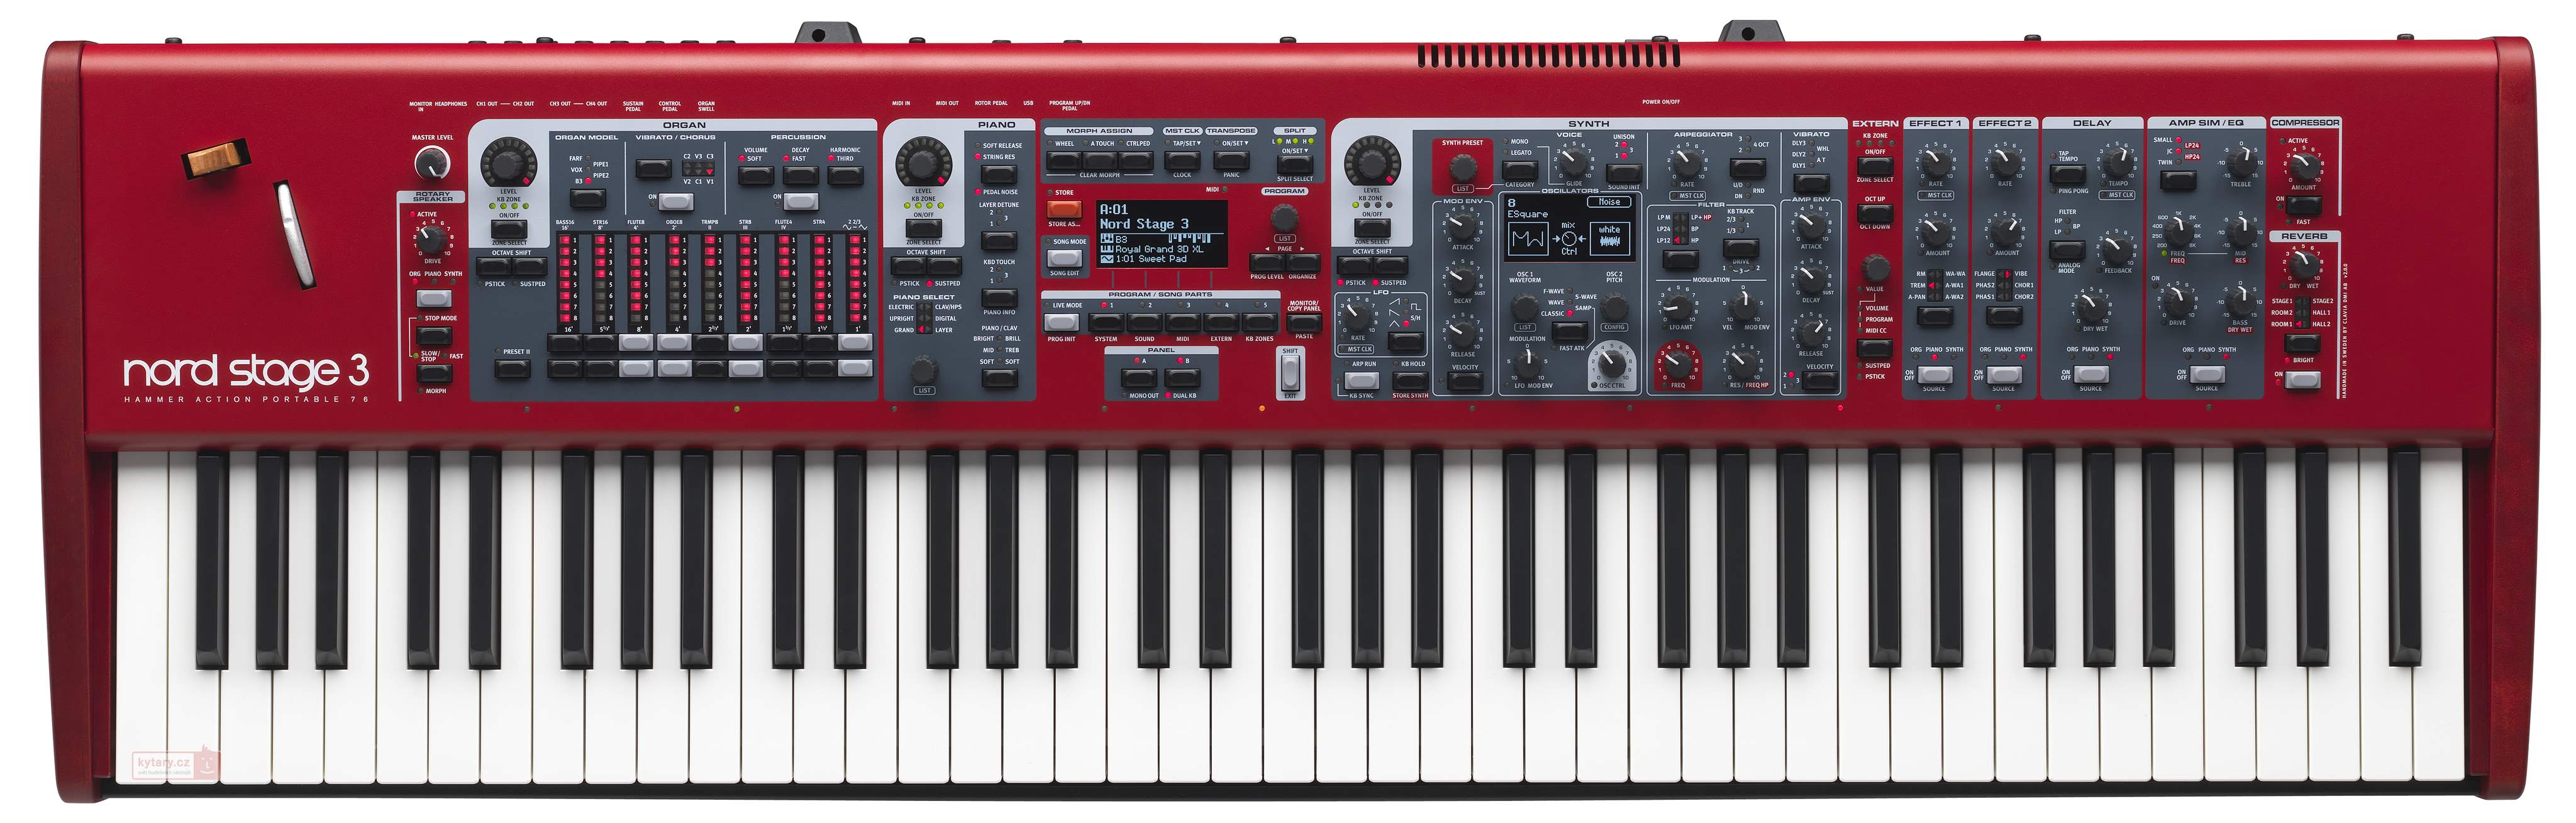
\includegraphics[width=1\textwidth]{HardwareStagepiano}
				\caption[Nord Stage 3 HP]{Nord Stage 3 HP}\label{fig:HardwareStagepiano}
			\end{figure}
		\subsection{Prostředí typu DAW}
			Prostředí typu DAW jsou určena převážně pro studiovou práci, tedy nahrávání, střih, míchání a postprodukci zvukového materiálu.
			K jejich využití je potřeba počítač nebo tablet. Klaviatury jsou připojeny přes MIDI rozhraní. Ke generování zvuku používají virtuální hudební nástroje.
			V prostředí lze používat více stop, kde každá stopa může používat různý virtuální nástroj a sadu efektů.
			Poskytuje také bohaté možnosti routování zvukového signálu.
			Nechybí ani integrace s klaviaturami a kontrolery, což usnadňuje práci a přispívá ke komfortu užívání.
			
			Ikdyž je prostředí typu DAW primárně určeno pro studiovou práci, může být vhodné i pro použití při živých vystoupeních.
			Jedná se však převážně o takový typ vystoupení, kdy má umělec předem pečlivě připravené celé představení.
			Flexibilita prostředí při samotném vystoupení je pak nízká.
			Lze sice docílit i flexibilního chování, nezbytná je však interakce uživatele s počítačem nebo tabletem. Při živém vystoupení
			je však taková interakce značně nevhodná, jelikož neposkytuje dostatečnou rychlost a preciznost ovládání.
			Navíc lze použít pouze omezené množství přednastavených zvuků, jelikož pro každý zvuk musí být zavedena zvláštní instance
			virtuálního nástroje, která čerpá systémové prostředky.
			
			\begin{figure}[H]
				\centering
				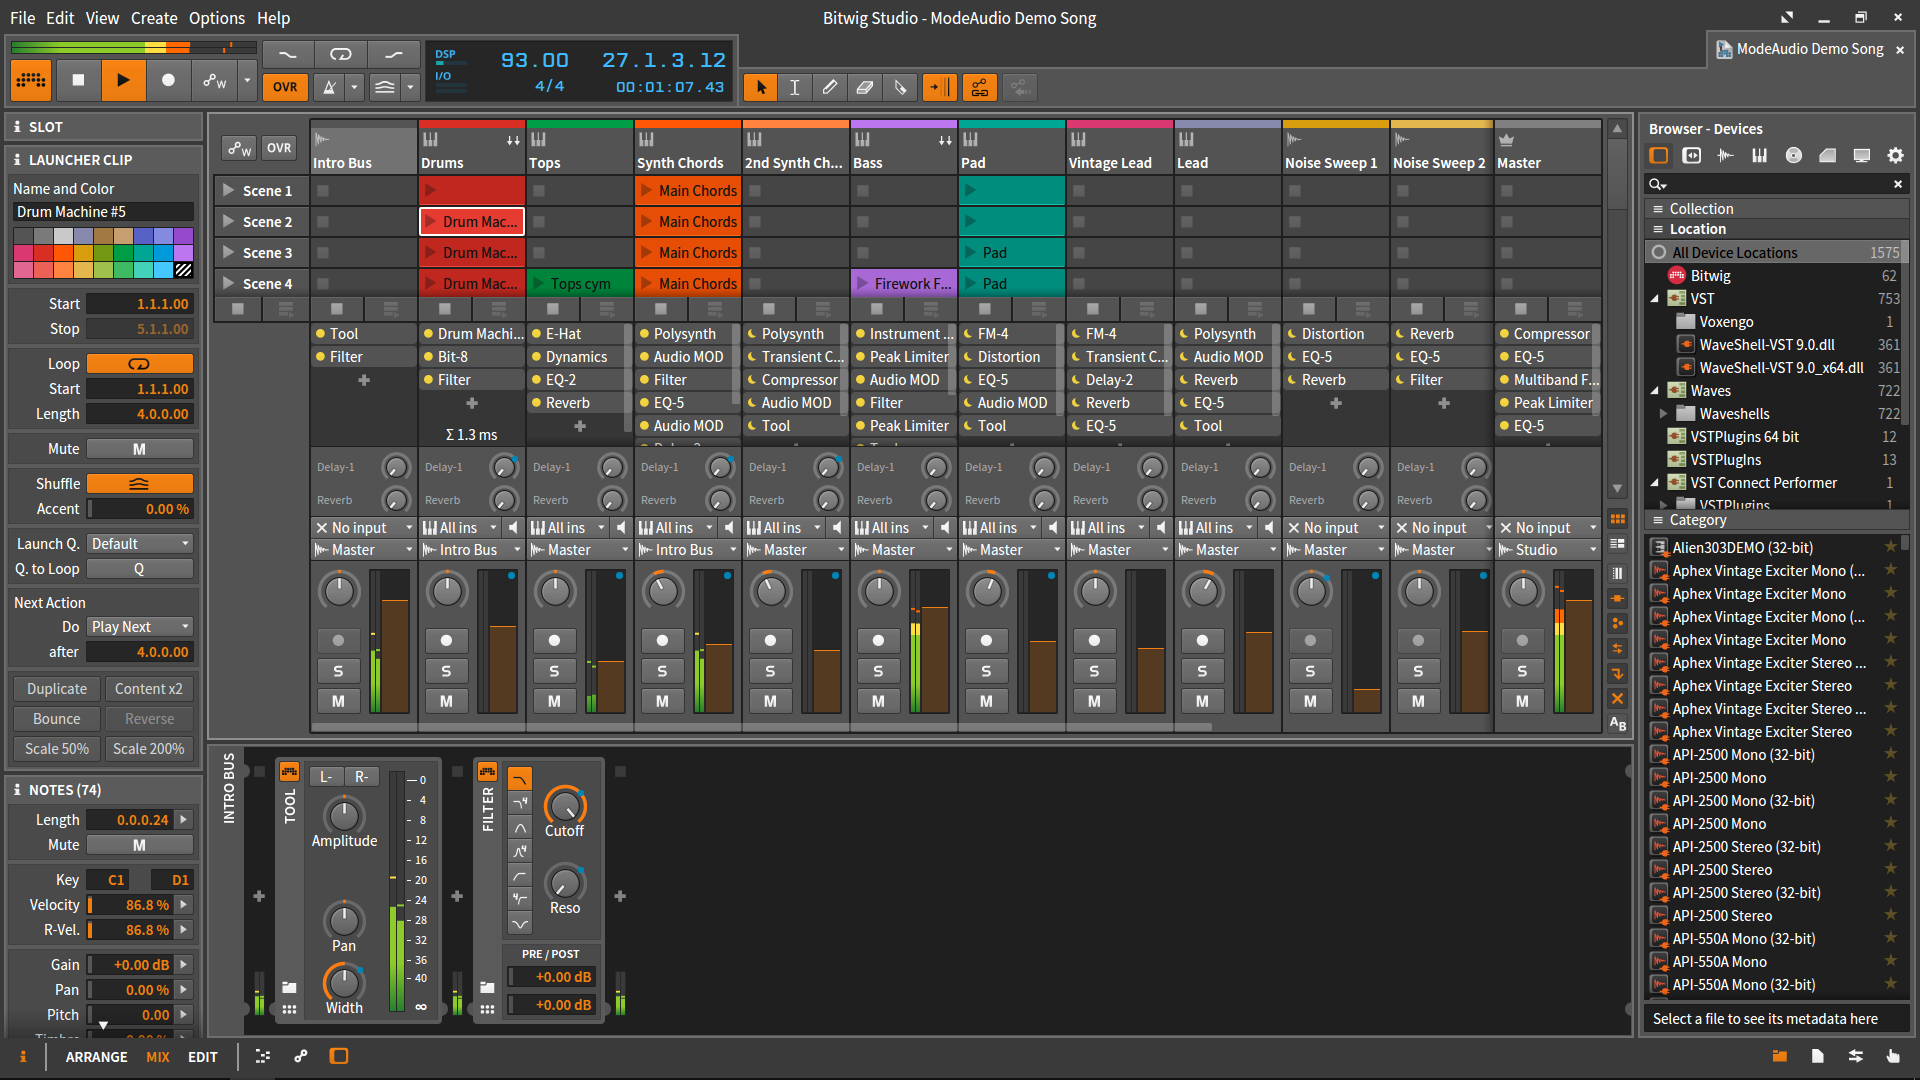
\includegraphics[width=1\textwidth]{DAW}
				\caption{Ukázka prostředí Bitwig Studio}\label{fig:DAW}
			\end{figure}
			
\clearpage
		\subsection{Prostředí pro živá vystoupení}
			S příchodem výkonných mobilních zařízení se začaly objevovat prostředí pro živá vystoupení.
			Jelikož jde o novou oblast a uživatelská základna není příliš početná, každé řešení přichází s unikátním přístupem. 
			Jasnou výhodou tohoto řešení je svoboda ve volbě zásuvných mdulů (pluginů)
			představujících virtuální nástroje a efekty.
			Další velkou výhodou je možnost připojit
			k systému více jednoduchých MIDI klaviatur.
			MIDI klaviatury vynikají oproti hardwarovým nástrojům
			nízkými pořizovacími náklady a nízkou hmotností.
			K systému využívající prostředí pro živá vystoupení
			lze připojit jakoukoliv MIDI klaviaturu. Umělec
			tak může v optimálním případě na zkoušky a vystoupení cestovat pouze s notebookem nebo tabletem, kde má uloženy veškeré zvuky a nastavení.
			
			Následuje výčet vlastností, které jsou pro většinu takových řešení společné.
			
			\begin{itemize}
				\item Snaha o optimalizaci využití systémových prostředků.
				\item Možnost vkládat vlastní skladby a jejich části.
				\item Možnost uložit konfiguraci zvuku pro skladbu a její část.
				\item Přítomnost filtrů, transformací a směrování MIDI zpráv.
				\item Podpora ovládání prostředí hardwarovým kontrolerem nebo tabletem.
				\item Multiplatformní podpora
				\item Podpora VST/VSTi API
			\end{itemize}
		
			V následující podkapitole bude zkoumán přední představitel prostředí pro živá vystoupení,
			software Cantabile od společnosti Topten Software.
			
			\subsubsection{Prostředí Cantabile}
				Software Cantabile od společnosti Topten Software představuje robustní řešení.
				Implementuje pokročilé optimalizace využití systémových prostředků a
				disponuje širokými možnostmi konfigurace, ovládání však není příliš intuitivní (viz obr. \ref{fig:Cantabile}).
				Prostředí umožňuje použití více klaviatur, jejich rozdělení na zóny a poskytuje bohaté možnosti
				pro směrování a transformaci MIDI zpráv, což zajišťuje vysokou flexibilitu.
				Způsob ukládání nastavení VST pluginů poskytuje více strategií.
				Cantabile se opírá o model uložení konfigurace pro uživatelem zadanou skladbu nebo její část.
				Integrace s hardwarovými kontrolery je z pohledu vstupu na vysoké úrovni, ovládacím prvkům lze přiřadit jakoukoliv 
				funkci programu. Z hlediska výstupu je však integrace omezená na obecnou úroveň, pro efektivní použití
				je třeba používat zároveň tablet nebo počítač.
				\begin{figure}[H]
					\centering
					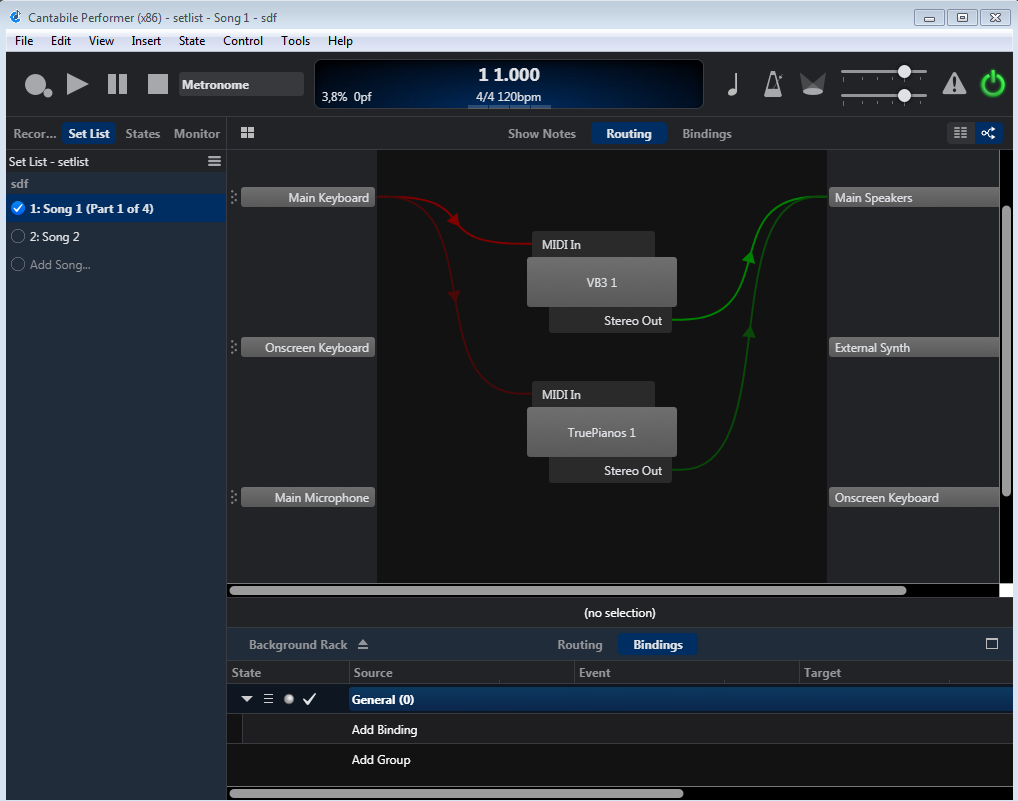
\includegraphics[width=1\textwidth]{Cantabile}
					\caption{Ukázka prostředí Cantabile}\label{fig:Cantabile}
				\end{figure}
		
	\section{Závěr}
		Z provedeného průzkumu je patrné, že existují různé možnoti řešení. Každé z nich řeší problém různým způsobem a má své výhody a nevýhody.
		Nebylo však nalezeno řešení, které by přinášelo možnost využití virtuálních hudebních nástrojů a integraci s hardwarovým kontrolerem tak,
		aby bylo dosaženo chování hardwarových hudebních nástrojů. Proto byla zvolena cesta návrhu vlastního řešení, které kombinuje přístup
		prostředí určených pro živá vystoupení a chování hardwarových nástrojů.

\chapter{Návrh vlastního řešení}
	\section{Architektura}
		Jelikož by bylo zbytečné realizovat celé řešení, bylo použito vzájemné propojení více technologií tak,
		aby vlastní implementace řešila pouze problémy přímo související s dosažením kýženého chování systému. V následujících podkapitolách
		budou rozebrány jednotlivé části architektury.
		
		\subsection{VST host}
			Každý virtuální hudební nástroj podporující VST API, tzv. VST plugin, potřebuje ke svému běhu hostitelské prostředí, tzv. VST host aplikaci, která API implementuje\cite{vstdoc}.
			
			VST API umožňuje pluginům generovat zvukovou vlnu na základě konfigurovatelných
			parametrů a vstupních dat, jako jsou MIDI události, či zvukový signál.
			Konfigurace parametrů virtuálního nástroje probíhá přes vlastní uživatelské rozhraní pluginu nebo přes hostitelskou aplikaci.
			Každý VST plugin poskytuje hostitelské aplikaci výčet dostupných parametrů a jejich vlastnosti.
			Zároveň je připravena i podpora tzv. presetů, které reflektují stav pluginu. Presety lze ovládat též prostřednictvím
			hostitelské aplikace.
			
			Hostitelská aplikace zároveň zajišťuje přenos zvukového signálu z pluginu, např. do zvukového rozhraní zařízení,
			a přenos MIDI zpráv do pluginu, např. z připojené klaviatury či kontroleru. Hostitelská aplikace musí vykazovat
			vysokou stabilitu, aby nedocházelo k výpadkům ve streamu zvukového signálu či k zahazování MIDI zpráv. Oblíbenou 
			technologií používanou k implementaci ovladačů zvukových zařízení při zachování nízké latence je technologie ASIO\cite{asio}.
			
			Jelikož by byla implementace funkcí hostitelského prostředí náročnou záležitostí, byl zvolen přístup využití
			již existující aplikace, která bude plnit úlohu VST hostitelského prostředí a bude ovládána externě naší vlastní aplikací.
			
		\subsection{OSC}		
			OSC představuje obecný a jednoduchý protokol určený pro přenos zpráv mezi multimediálními zařízeními a aplikacemi\cite{osc}.
			Obsah zprávy je složen z adresy ve tvaru řetězce a argumentů několika typů.
			Zprávy jsou přenášeny typicky přes UDP protokol. Multimediální aplikace často poskytují možnost oboustranné integrace
			se službami třetích stran právě přes OSC protokol.

		\subsection{HW kontroler}
			Hardwarový kontroler slouží k ovládání multimediálních aplikací nebo zařízení. V naprosté většině případů k přenosu používá MIDI protokol
			a bývá připojen přes rozhraní USB nebo MIDI. Kontroler navíc může být vybaven prezentačními prvky, jako jsou LED indikátory, displej apod.

		\subsection{Automap}
			Protokol Automap od společnosti Novation je postavený nad protokolem MIDI, využívá kombinaci zpráv typu CC a SysEx \cite{midi}\cite{automap}.
			Slouží k integraci multimediálních aplikací se skupinou kontrolerů od společnosti Novation. Existují implementace pro 
			přední DAW prostředí.

		\subsection{Vlastní aplikace}
			Cílem vlastní aplikace je propojení všech komponent tak, aby bylo dosaženo požadované funkcionality.
			Aplikace bude ovládat VST hostitelské prostředí a v něm obsažené nástroje a efekty s využitím OSC protokolu.
			S hardwarovým kontrolerem bude aplikace obousměrně integrována přes protokol Automap.
			K dispozici bude též desktopové uživatelské rozhraní sloužící ke konfiguraci zvuků, presetů a dalších nastavení.
\clearpage
		\subsection{Závěr}
			Na diagramu \ref{fig:Architecture} je zobrazena architektura systému.
			\begin{figure}[H]
				\centering
				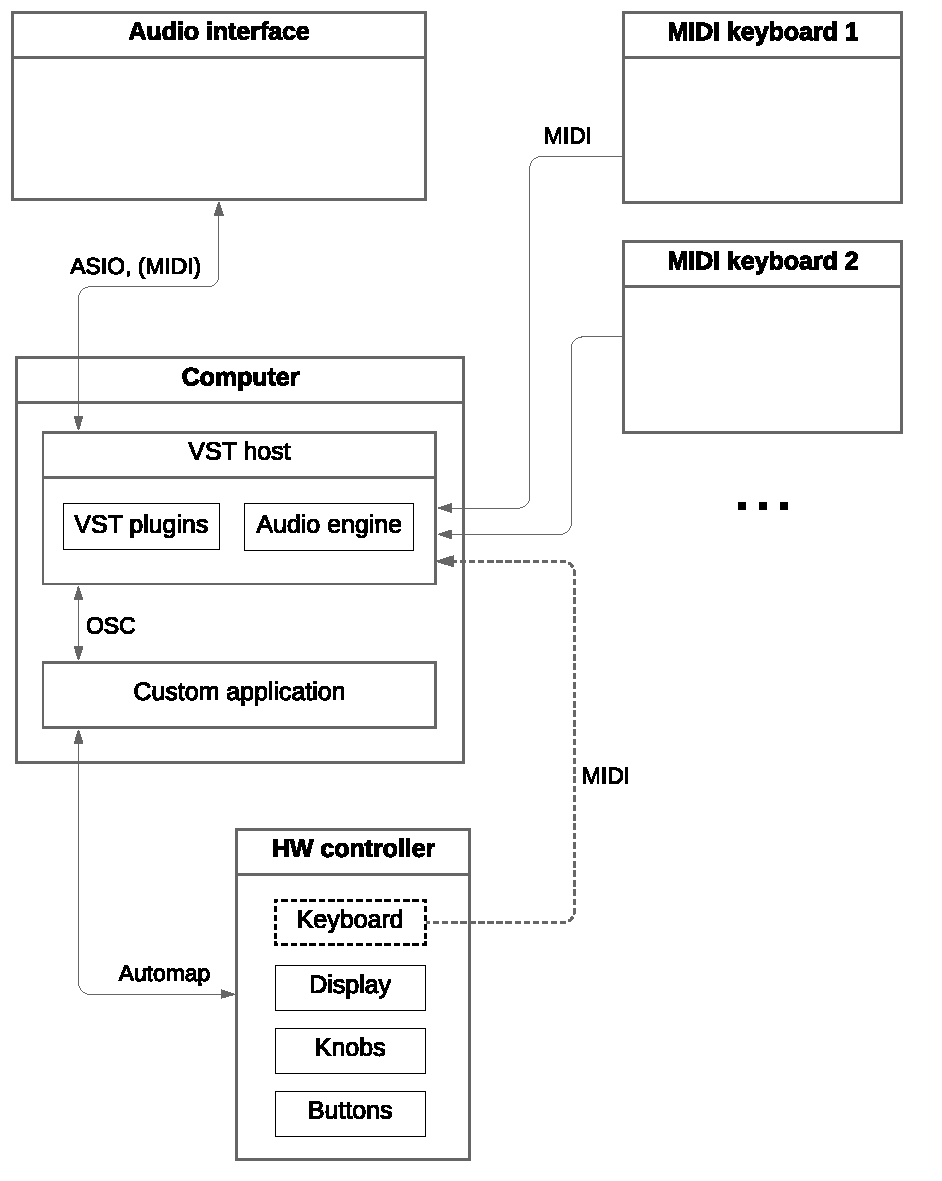
\includegraphics[width=1\textwidth]{Architecture}
				\caption{Architektura řešení}\label{fig:Architecture}
			\end{figure}
\clearpage
	\section{Analýza kompatibility}
		Na počátku byla provedena analýza kompatibility jednotlivých komponent. 
		
		\subsection{HW kontroler}
		Při analýze kompatibility kontroleru za použití modelu Novation SLMkII 49 bylo zjištěno, že
		kontroler připojený přes USB sice exportuje rozhraní pro komunikaci přes protokol Automap,
		ale toto rozhraní nehlásí systému příslušnou třídu USB zařízení. Podle zachycené sériové komunikace
		se ukázalo, že formát přenášených dat přesto odpovídá třídě USB pro MIDI zařízení\cite{usbmidi}.
		
		\subsection{VST host}
		Jako hostitelská aplikace pro VST pluginy byl testován program Bidule of společnosti Plogue.
		Z anlýzy vyplynulo, že poskytuje bohaté možnosti ovládání přes kombinaci protokolů OSC a UDP.
		Program přes OSC umožňuje spouštět důležité akce, lze navíc přijímat a odesílat hodnoty všech VST pluginů a interních modulů.
		Data jsou uložena ve formátu XML, ze kterého lze snadno získat veškeré informace o uloženém projektu.
		
	\section{Zvolené technologie}
		Na základě analýzy kompatibility byl za hardwarový kontroler zvolen model Novation SLMkII 49, jako VST hostitelskou aplikací byl zvolen program Bidule od společnosti Plogue.
		Pro zajištění nízkoúrovňové komunikace s kontrolerem byl zvolen univerzální USB ovladač WinUSB pro platformu Windows.
	
		Při výběru technologií pro implementaci vlastní aplikace byly zohledněny následující požadavky:
		\begin{itemize}
			\item Možnost low-level komunikace přes USB
			\item Podpora komunikace přes UDP
			\item Podpora asynchronního kódu na vysoké úrovni
			\item Nenáročná tvorba UI
			\item Stabilita a rychlost odezvy
		\end{itemize}
			
		Pro implementaci vlastní aplikace byl zvolen programovací jazyk TypeScript, jehož kód je kompilován do jazyka JavaScript.

		Dále byl zvolen framework Electron, který poskytuje možnost tvorby desktopových aplikací za použití jazyka JavaScript.
		Při spuštění aplikace vytvořené ve frameworku Electron je spuštěn na pozadí tzv. hlavní proces.
		Hlavní proces vytváří další vedlejší nezávislé procesy, které slouží k zobrazení oken s webovým prohlížečem, kde je načtena klientská část aplikace.
		Ke komunikaci mezi hlavním a vedlejšími procesy framework poskytuje jednoduché rozhraní.

		Komunikaci mezi aplikací a hardwarovým kontrolerem lze implementovat pouze v hlavním procesu. Původním záměrem bylo tedy využítí architektonického vzoru tlustý klient. 
		Hlavní proces by fungoval pouze jako proxy pro protokoly OSC a Automap mezi příslušnými komponentami a klientskou částí aplikace (diagram \ref{fig:AppArchitectureA}).
		Při testování bylo zjištěno, že rozhraní pro komunikaci mezi hlavním a vedlejšími vlákny není pro tento účel dostatečně rychlé a nemá dostatečně rychlou odezvu.
		Jako řešení tohoto problému bylo zvoleno rozdělení aplikace na serverovou a klientskou část, kde mezi oběmi stranami nebude docházet k objemné komunikaci citlivé na dobu odezvy.
		Jelikož lze předpokládat, že velká část stavu aplikace bude sdílená serverovou i klientskou částí, byl vybrán pro obě části framework pro vývoj webových aplikací Angular a knihovna NGXS představující framework pro řízení stavu podle patternu CQRS\cite{cqrs}, který vychází ze vzoru CQS\cite{cqs}. Výhodou je pak možnost automatické synchronizace stavu mezi serverovou a klientskou částí (diagram \ref{fig:AppArchitectureB}).
		



		\begin{figure}
			\centering		
			\subfloat[Původní návrh]{{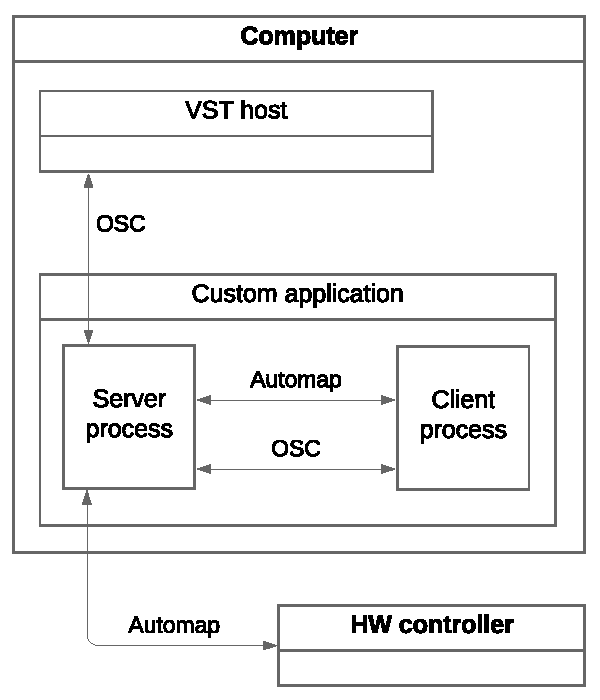
\includegraphics[width=5.8cm]{Dip-AppArchitecture1}												\label{fig:AppArchitectureA} }}
			\qquad
			\subfloat[Optimalizovaný návrh]{{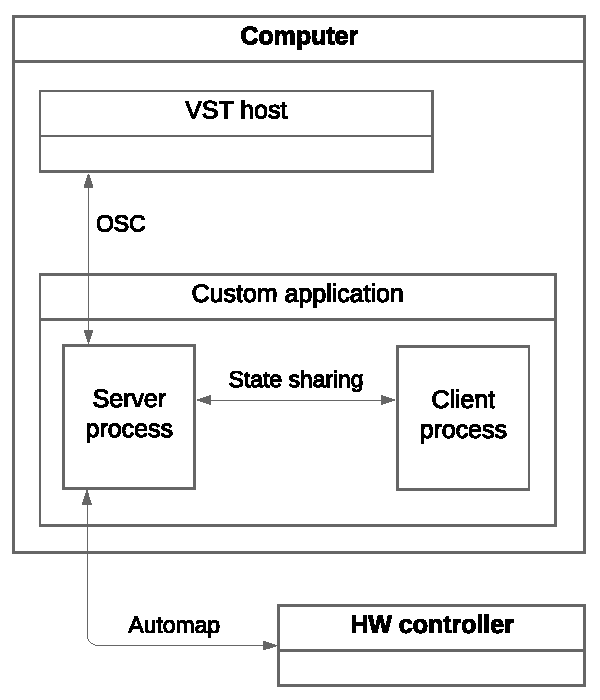
\includegraphics[width=5.8cm]{Dip-AppArchitecture2}
				\label{fig:AppArchitectureB} }}
			\caption{Srovnání původního a konečného návrhu architektury aplikace.}
			\label{fig:AppArchitecture}
		\end{figure}
		
		Pro klientskou část byla použita knihovna \texttt{Angular Material UI}, která poskytuje základní prvky pro tvorbu uživatelského rozhraní.

		Pro servrovou část byla využita knihovna \texttt{tessel/node-usb}, jejíž úlohou je zpřístupnění funkcí knihovny \texttt{libusb}, která poskytuje možnost low-level komunikace s USB zařízeními\cite{libusb}.
		V serverové části též byla využita knihovna \texttt{node-osc}, která umožňuje komunikaci přes OSC a UDP protokol.
		
	\section{Funkční požadavky}
		Při návrhu řešení byly určeny následující funkční požadavky.
	
		V aplikaci bude možné používat více projektů programu Bidule. Bude k dispozici rozhraní pro správu projektů, kde bude možné
		zadat cestu k uloženému projektu a název projektu. Je možné načíst a zavřít projekt. Veškerá nastavení kromě globálních se budou ukládat 
		pro každý projekt zvlášť. Po načtení projektu dojde k automatickému importu konfigurace projektu Bidule.
		
		Vrstvou se rozumí skupina VST pluginů definovaná v projektu programu Bidule. Manuálem se rozumí skupina vrstev a představuje připojenou klaviaturu.

		V rámci aplikace bude možné zobrazit seznam dostupných nástrojů a efektů. Seznam nástrojů a efektů bude importován z konfigurace projektu Bidule.
		U nástrojů a efektů bude možné vytvořit snímek všech parametrů pluginu, který bude považován za výchozí a bude načten při načtení projektu nebo po přepnutí zvuku. V rámci obou seznamů bude též možné otevřít uživatelské rozhraní VST pluginu, či zobrazit jeho dostupnost v jednotlivých vrstvách. Pro nástroje bude možnost definovat více pojmenovaných stránek mapování, pro efekt bude možné zadat právě jednu stránku mapování s volbou hlavního mapování.

		Editor stránek mapování bude poskytovat možnost konfigurace mapování parametrů VST pluginu na enkodéry kontroleru.
		V rámci jedné stánky mapování bude možné ke každému enkodéru přiřadit právě jeden parametr VST pluginu a zadat tak až 8 různých mapování.
		Při volbě parametru pluginu bude možné použít tzv. funkce learn, kdy lze ovládaný parametr vybrat přímo v uživatelském rozhraní pluginu.
		Bude možné zadat název mapování.
		Pro každé mapování budou k dispozici následující strategie:
		\begin{itemize}
			\item\label{LinearMappingStrategy} \textbf{Lineární} - Tato strategie bude umožňovat určit lineární vztah mezi hodnotou enkodéru na hardwarovém kontroleru 
			a hodnotou parametru příslušného pluginu. Bude možné zadat rozsah hodnot zobrazených na displeji, rozsah hodnot parametru VST pluginu, invertovat
			průběh a zadat suffix pro zobrazení na displeji. Rozsah hodnot parametrů pluginu bude možné nastavovat i přes tzv. learn metodu, která 
			umožňuje hodnoty zvolit přímo v prostředí VST pluginu. Na LED prstencích rotačních enkodérů kontroleru bude hodnota parametru indikována lineárně na celém rozsahu enkodéru.
			
			\item \textbf{Lineární s položkovým zobrazením} - Jedná se o rozšíření lineární strategie s možností zadání položek, které
			budou zobrazeny na displeji v závislosti na hodnotě parametru pluginu. Každá položka bude určena názvem a hraniční hodnotou parametru VST pluginu.
			Položky bude možné přidávat i za pomoci tzv. learn metody, kdy je možné zadat hraniční hodnotu přímo v prostředí VST pluginu.

			\item \textbf{Seznam} - Za použití této strategie bude možné definovat seznam položek obsahujících název a hodnotu parametru VST pluginu.
			Oproti lineární strategii s položkovým zobrazením bude probíhat změna hodnoty parametru VST pluginu skokově. Při reflektování změn hodnoty parametru bude zobrazena
			položka, která je aktuální hodnotě parametru nejblíže.
		\end{itemize}
		
		V editoru presetů bude možné zadat až 8 kategorií zvuků, které bude možné řadit a přejmenovat.
		Pro každou kategorii bude možné přidat nový preset, či duplikovat stávající. Preset určuje použitý VST plugin,
		strategii inicializace pluginu vč. její konfigurace, rozdílovou sadu hodnot parametrů pluginu a rozdílovou sadu hodnot parametrů efektů vrstvy.
		Rozdílová sada bude pro danou vrstvu vytvářena při změně v parametrech pluginu v době, kdy je preset aktivní. Zaznamenanou sadu bude možné pro aktivní preset uložit.
		V rámci inicializace VST pluginu budou k dispozici následující strategie:
		\begin{itemize}
			\item \textbf{Snímek všech parametrů} - V této strategii bude možné pořídit snímek hodnot všech parametrů VST pluginu. Snímek bude načten při načtení presetu.
			\item \textbf{Zpráva typu Program Change} - Tato strategie zajistí odeslání MIDI zprávy typu Program Change do patřičného VST pluginu.
			\item \textbf{Načtení nativního VST presetu} - Za použití této strategie dojde k načtení nativního presetu VST pluginu. Nativní presety je možné editovat
			v hostitelské aplikaci či přímo v pluginu.
		\end{itemize}
		Pro každou vrstvu může být aktivní právě jeden preset. Po načtení presetu bude 
		pro danou vrstvu aplikovaná inicizalizační strategie na virtuální nástroj a budou načteny rozdílové sady hodnot parametrů nástroje a efektů.
		Vlastnosti presetu bude možné upravit, či preset odstranit.
	
		Za použití kontroleru bude možný výběr kategorie a stránkovaný výběr presetu v rámci dané kategorie. Zároveň bude k dispozici
		historie posledních použitých presetů vč. jejich stavů pro každou vrstvu.
		Hodnoty parametrů pluginů bude možné ovládat rotačními enkodéry kontroleru. Hodnoty budou indikovány LED prstencem enkodéru a grafickým výstupem na displeji podle konfigurace strategie mapování.
		V rámci ovládání parametrů nástrojů bude k dispozici
		zobrazení stránky mapování daného presetu. Pro ovládání parametrů efektů bude k dispozici agregované zobrazení, kde bude zobrazena
		hlavní položka stránky mapování pro každý efekt, který je v dané vrstvě dostupný. Bude možné ovládat i všechny parametry efektu.
		Kontroler uživateli umožní přepínat a indikovat právě ovládanou vrstvu. 
		Za pomocí posuvných prvků kontroleru bude možné ovládat hlasitosti jednotlivých vrstev.
		K dispozici bude též ovládání hlavní hlasitosti a tlačítko pro ukonćení všech znějících tónů.
	
	\section{Doménový model}
		Z analýzy požadavků byl navržen doménový model (viz obr. \ref{fig:DomainModel}),
		který zobrazuje entity problémové domény a jejich vzájemné vztahy.
		\begin{figure}
			\centering
			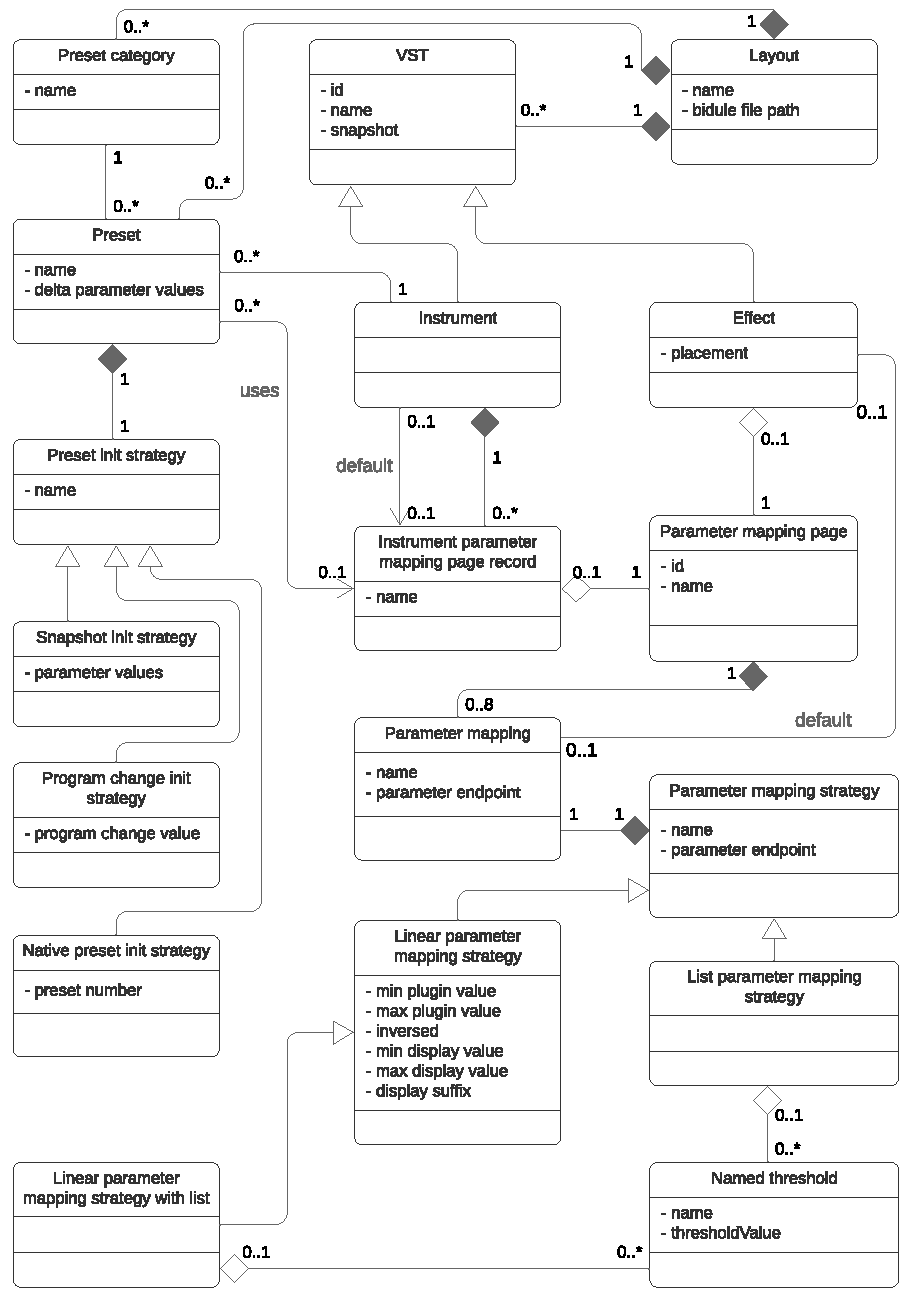
\includegraphics[width=1\textwidth]{DomainModel}
			\caption{Doménový model}\label{fig:DomainModel}
		\end{figure}		

	\section{Struktura projektu Bidule}\label{sec:bidule-components}
		Aby mohly být projekty uložené v programu Bidule načteny ve vlastní aplikaci, je třeba definovat strukturu
		projektů. Projekt vytvořený v programu Bidule se skládá z modulů, které jsou uspořádány do stromové struktury
		a jsou vzájemně propojeny. Modulem může být např. VST plugin, vstupně-výstupní rozhraní pro audio nebo MIDI.
		Program Bidule též poskytuje množství interních modulů. Moduly lze agregovat do samostatných celků a vytvářet tak
		vlastní znovupoužitelné moduly. V následujících podkapitolách budou rozebrány jednotlivé části architekury projektu programu Bidule.
		Příklad možné architektury lze vidět na diagramu \ref{fig:BiduleComponents}.
		
		\begin{figure}
			\centering
			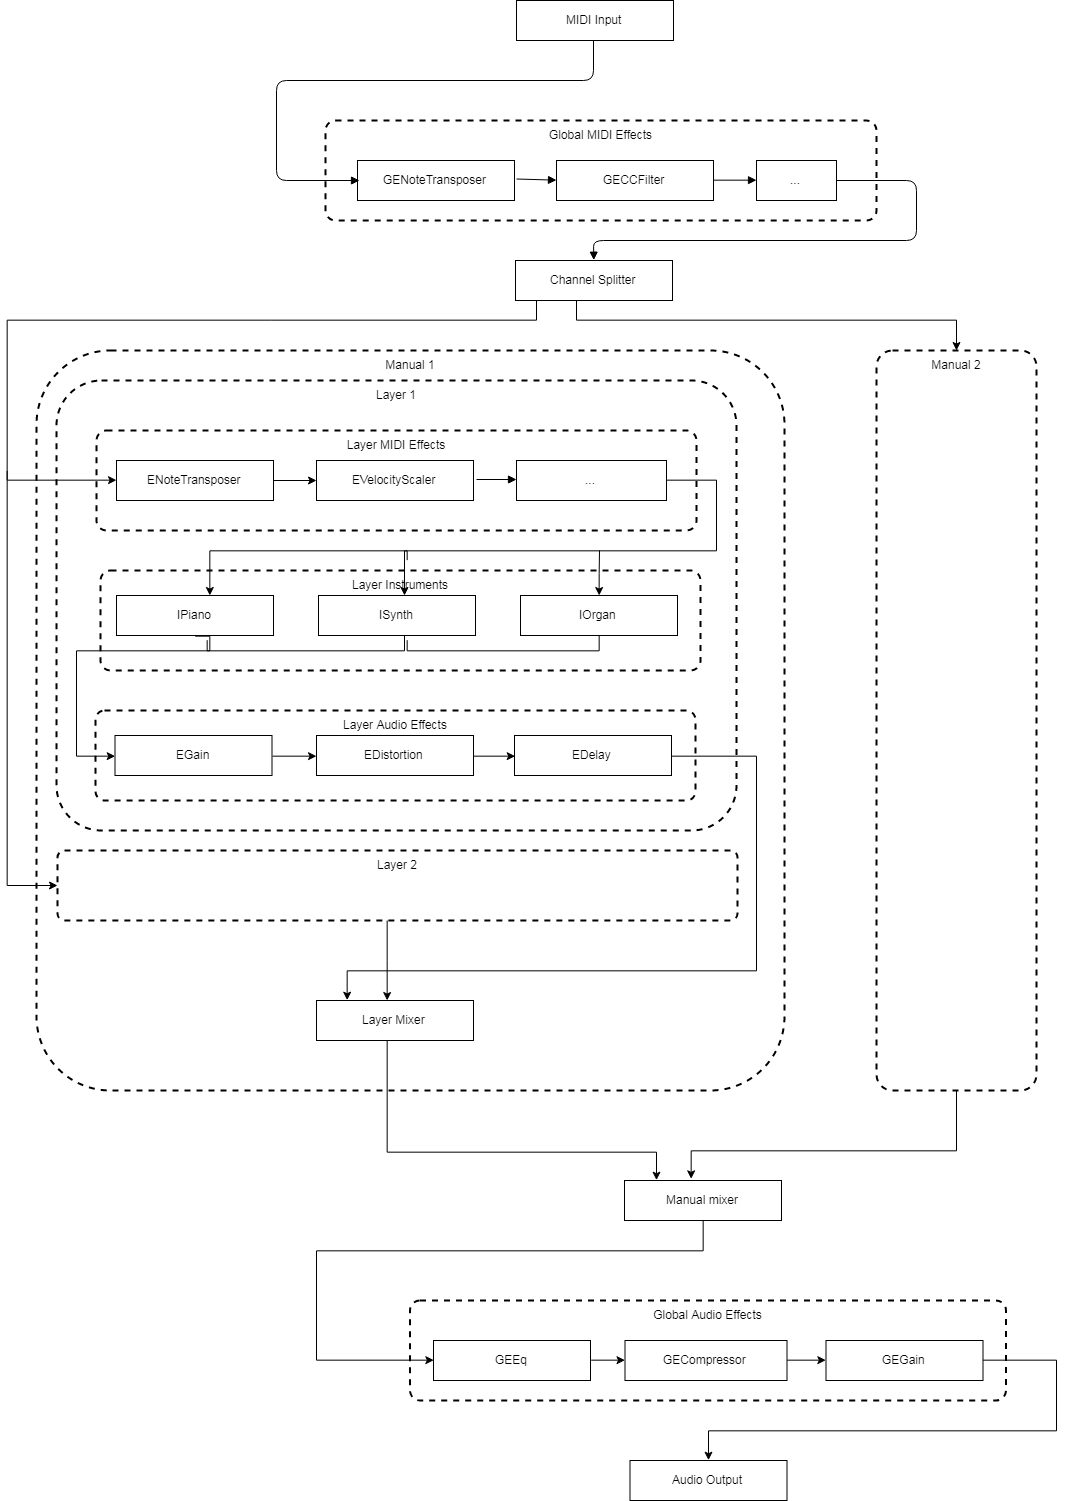
\includegraphics[width=1\textwidth]{BiduleComponents}
			\caption{Ukázka architektury projektu Bidule}\label{fig:BiduleComponents}
		\end{figure}
			
		\subsection{Modul manuálu}\label{sec:Bidule-Manual}
			Modul manuálu se skládá ze skupiny vrstev (viz kapitolu \ref{sec:Bidule-Layer}) a modulu pro zajištění smíchání zvukového signálu
			jednotlivých vrstev. Představuje konfiguraci dostupnou pro připojenou klaviaturu. Každá klaviatura může mít různý počet
			vrstev. Doporučeno je však použití stejné konfigurace pro všechny manuály kvůli snazší orientaci uživatele.
			V projektu může být zadán jeden až čtyři manuály.

		\subsection{Modul vrstvy}\label{sec:Bidule-Layer}
			Modul vrstvy představuje sadu vstupních efektů, virtuálních nástrojů a výstupních efektů.
			Skupina vrstev je součástí modulu manuálu (viz kapitolu \ref{sec:Bidule-Manual}).
			Manuál může obsahovat jednu až čtyři vrstvy.
			Každá vrstva může obsahovat různé moduly. Pro jednodušší orientaci uživatele je však doporučeno
			uchovat všehcny dostupné vrstvy ve stejné konfiguraci, a to i mezi jednotlivými manuály.
			
		\subsection{Globální efekty}
			V projektu je možné definovat vstupní a výstupní efekty, které budou k dispozici nezávisle na vrstvě
			a budou aplikovány na veškerá vstupní a výstupní multimediální data. Příkladem takového efektu může být
			transpozice tónů nebo ekvalizace zvukového výstupu. Vstupní a výstupní efekty jsou rozděleny do dvou skupin.
			Projekt může obsahovat až 8 vstupních a 8 výstupních efektů.

		\subsection{Vstupně-výstupní rozhraní}
			V projektu musí být k dispozici alespoň jedno MIDI vstupní zařízení a jedno zvukové vstupně-výstupní zařízení.
			Vstup z MIDI zařízení je směrován do skupiny komponent představujících globálních MIDI efekty.
			Výstup ze skupiny komponent představující globální zvukové efekty je pak směrován do výstupního zvukového zařízení.
			V případě potřeby lze také směrovat vstup ze zvukového zařízení do nástrojů a efektů, které podporují zpracování
			zvukového signálu.
			
		\subsection{Propojení modulů}
			Jelikož musí být zachována variabilita směrování MIDI zpráv, celý systém pracuje pouze s jedním zdrojem MIDI zpráv.
			Každá MIDI zpráva má určené číslo kanálu, které může nabývat 16 různých hodnot.
			U zdrojových MIDI zprávy lze v programu Bidule libovolně přemapovat kanál pomocí interních modulů, např. na základě rozsahu klaviatury, připojeného manuálu apod.
			Podle kanálu zprávy je pak zpráva směrována do příslušného modulu manuálu. Smíchání zvukového signálu ze všech modulů manuálu je zajištěno interním modulem programu Bidule.
	
			Celé propojení jednotlivých modulů lze vidět na obr. \ref{fig:BiduleComponents}.

	\section{Desktopové uživatelské rozhraní}
		Při návrhu uživatelského rozhraní desktopové aplikace byl sestrojen následující seznam obrazovek.
		\begin{mylist}
			\begin{enumerate}[label=\textbf{D\arabic*.}]
				\item Seznam projektů
				\item Editace projektu
				\item Seznam nástrojů
				\item Zobrazení dostupnosti nástroje (obr. \ref{fig:DesktopUI-InstrumentAvailability})
				\item Správce mapování parametrů pluginu pro nástroje (obr. \ref{fig:DesktopUI-InstrumentParamMapping})
				\item Seznam efektů (obr. \ref{fig:DesktopUI-EffectList})
				\item Zobrazení dostupnosti efektu
				\item Správce mapování parametrů pluginu pro efekty	(obr. \ref{fig:DesktopUI-EffectParamMapping})		
				\item Správce presetů
				\item Editace presetu
			\end{enumerate}
			\caption{Seznam obrazovek desktopového uživatelského rozhraní aplikace}\label{list:DesktopUIScreen}		
		\end{mylist}
	
		Pro vybrané obrazovky byly sestrojeny drátěné modely 
		(obr. \ref{fig:DesktopUI-EffectList}, \ref{fig:DesktopUI-InstrumentAvailability}, 
		\ref{fig:DesktopUI-EffectParamMapping}, \ref{fig:DesktopUI-InstrumentParamMapping}).
		
		\begin{figure}
			\centering
			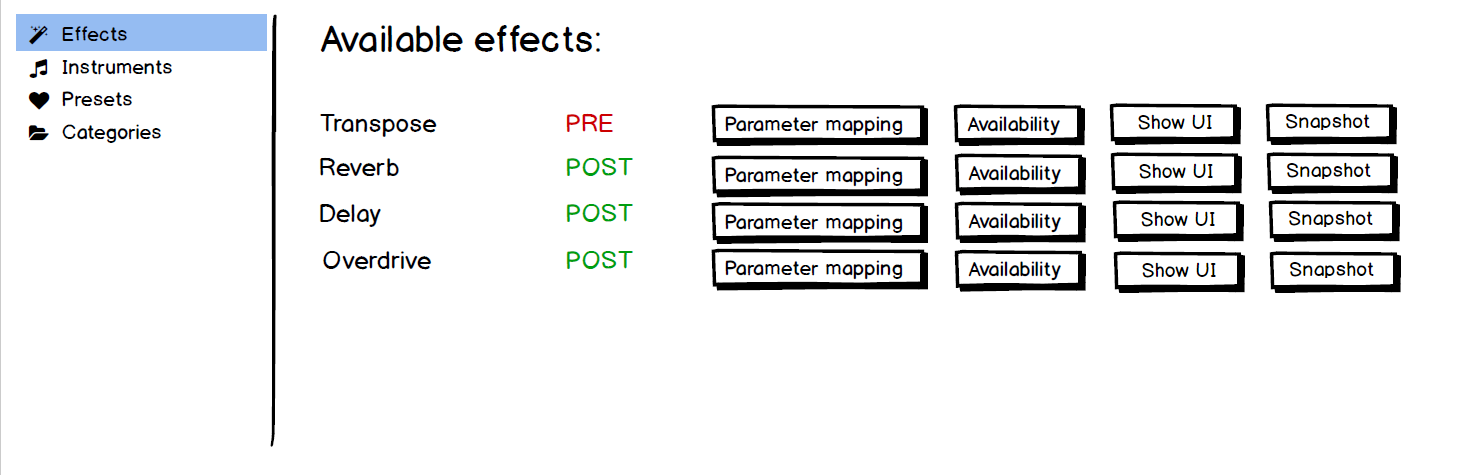
\includegraphics[width=1\textwidth]{DesktopUI-EffectList}
			\caption{Drátěný model obrazovky \texttt{D6} (seznam efektů)}\label{fig:DesktopUI-EffectList}
		\end{figure}
		\begin{figure}
			\centering
			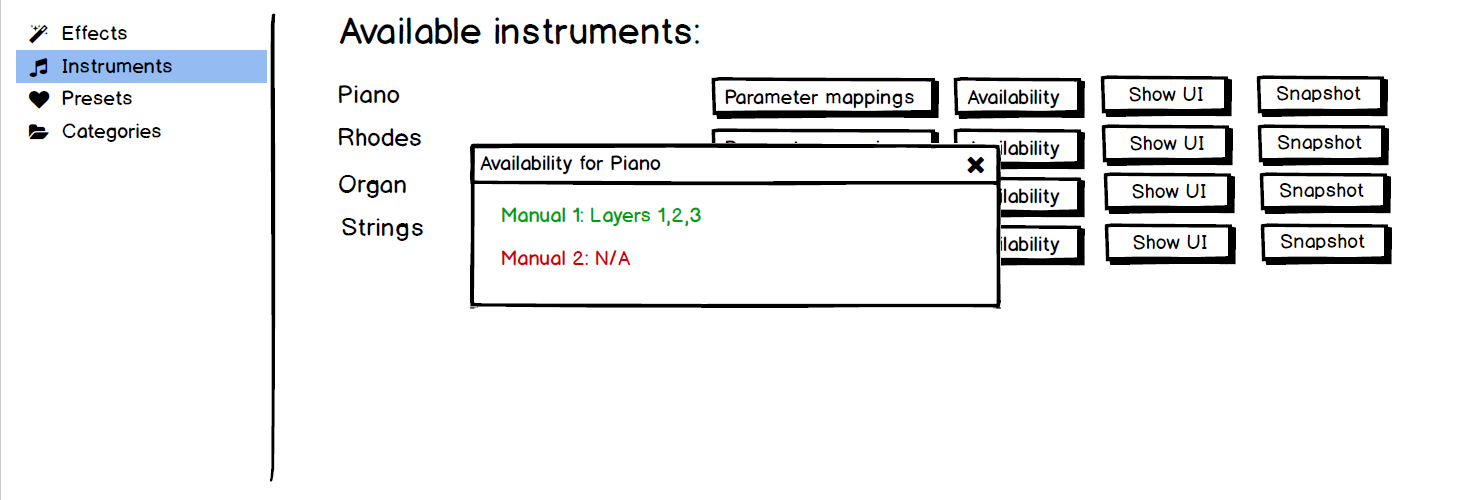
\includegraphics[width=1\textwidth]{DesktopUI-InstrumentAvailability}
			\caption{Drátěný model obrazovky \texttt{D4} (zobrazení dostupnosti) nástroje}\label{fig:DesktopUI-InstrumentAvailability}
		\end{figure}
		\begin{figure}
			\centering
			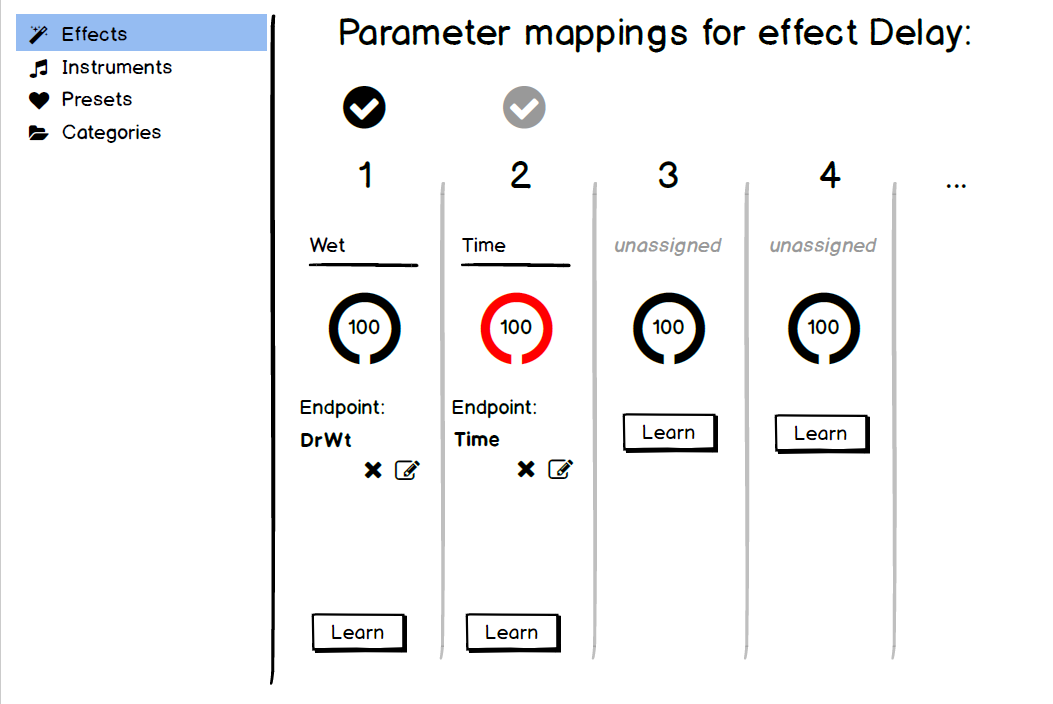
\includegraphics[width=1\textwidth]{DesktopUI-EffectParamMapping}
			\caption{Drátěný model obrazovky \texttt{D8} (správce mapování parametrů pluginu pro efekty)}\label{fig:DesktopUI-EffectParamMapping}
		\end{figure}
		\begin{figure}
			\centering
			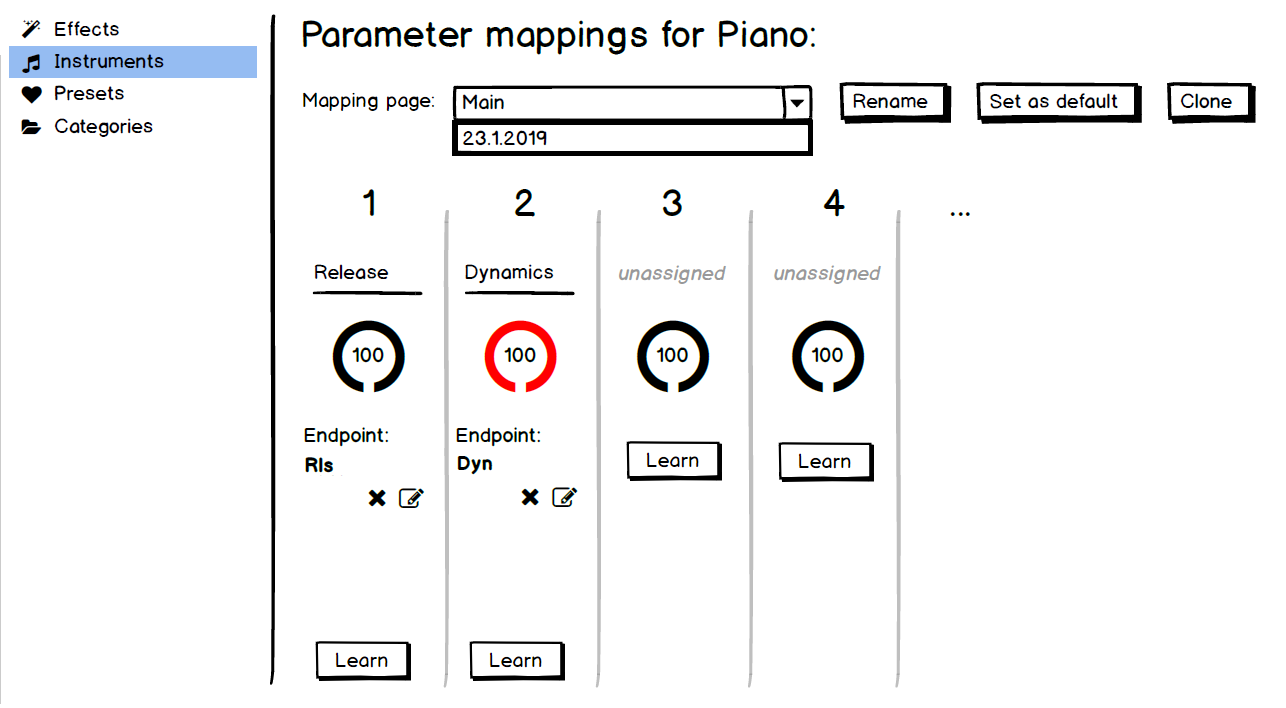
\includegraphics[width=1\textwidth]{DesktopUI-InstrumentParamMapping}
			\caption{Drátěný model obrazovky \texttt{D5} (správce mapování parametrů pluginu pro nástroje)}\label{fig:DesktopUI-InstrumentParamMapping}
		\end{figure}

	\vfill
	\pagebreak
	\section{Uživatelské rozhraní kontroleru}
		
		Jelikož byl v řešení vybrán hardwarový kontroler podporující protokol Automap,
		bylo navrženo uživatelské rozhraní pro celou skupinu kontrolerů společnosti Novation
		podporující tento protokol. Všechna taková zařízení disponují téměř shodným 
		rozvržením prvků (obr. \ref{fig:AutomapUI}).
		
		\begin{figure}[H]
			\centering
			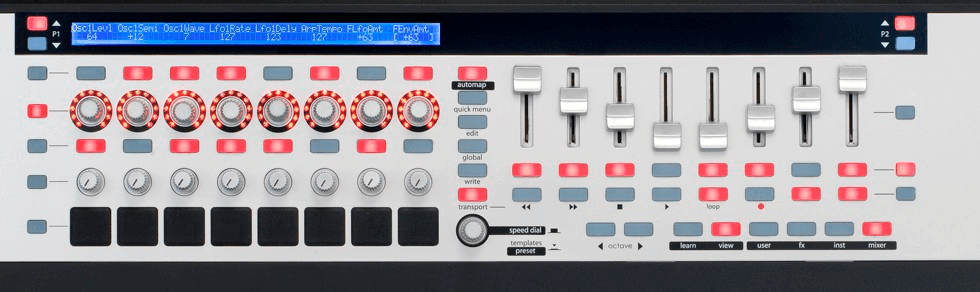
\includegraphics[width=1\textwidth]{AutomapUI}
			\caption{Ovládací panel zařízení od společnosti Notvation podporující protokol Automap.}\label{fig:AutomapUI}
		\end{figure}	

		V rámci návrhu uživatelského rozhraní pro hardwarový kontroler byl kladen důraz na oblast ovládacích prvků umístěných kolem displeje.
	 	Seznam \ref{list:ControllerUIScreen} shrnuje klíčové obrazovky hardwarového kontroleru. Jednotlivé obrazovky budou diskutovány
	 	v dalších podkapitolách.
		\begin{mylist}
			\begin{enumerate}[label=\textbf{C\arabic*.}]
				\item Procházení presetů (obr. \ref{fig:ControllerUI-PresetSwitch})
				\item Ovládání parametrů nástroje (obr. \ref{fig:ControllerUI-PresetDetail})
				\item Souhrnné ovládání efektů  (obr. \ref{fig:ControllerUI-EffectOverview})
				\item Ovládání parametrů efektu (obr. \ref{fig:ControllerUI-EffectDetail})
			\end{enumerate}
			\caption{Seznam obrazovek desktopového uživatelského rozhraní aplikace}\label{list:ControllerUIScreen}		
		\end{mylist}
		
		\begin{sidewaysfigure}
			\centering
			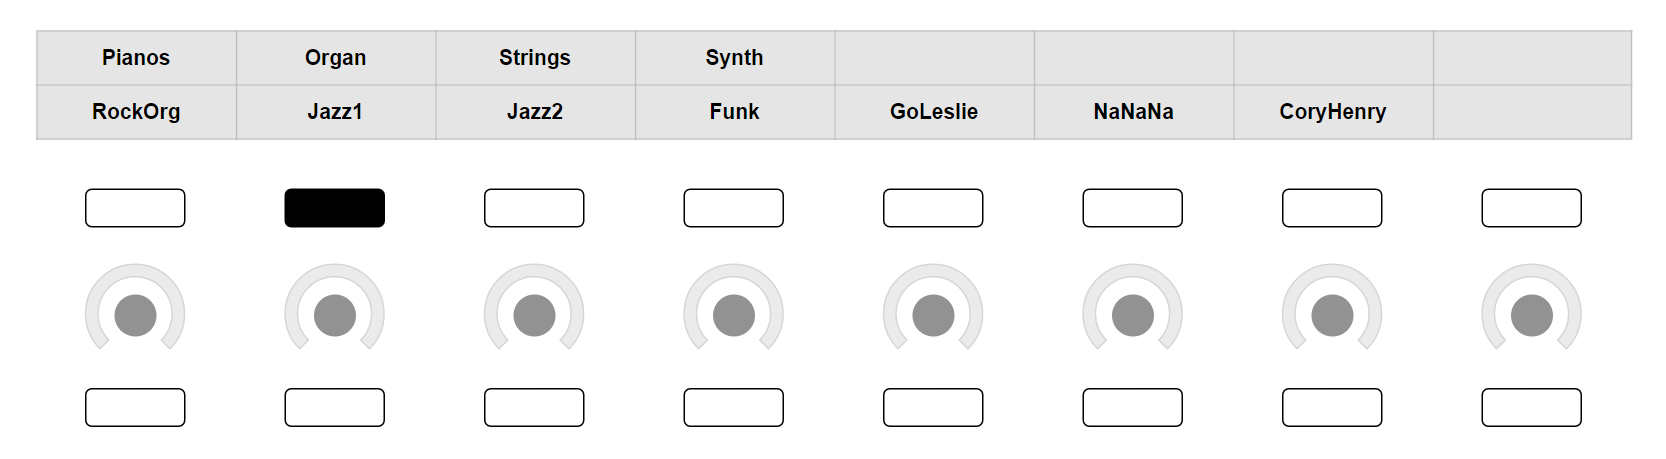
\includegraphics[width=0.9\textwidth]{ControllerUI-PresetSwitch}
			\caption{Drátěný model obrazovky \texttt{C1} (procházení presetů)}
			\label{fig:ControllerUI-PresetSwitch}			
			\vspace{1.2cm}
			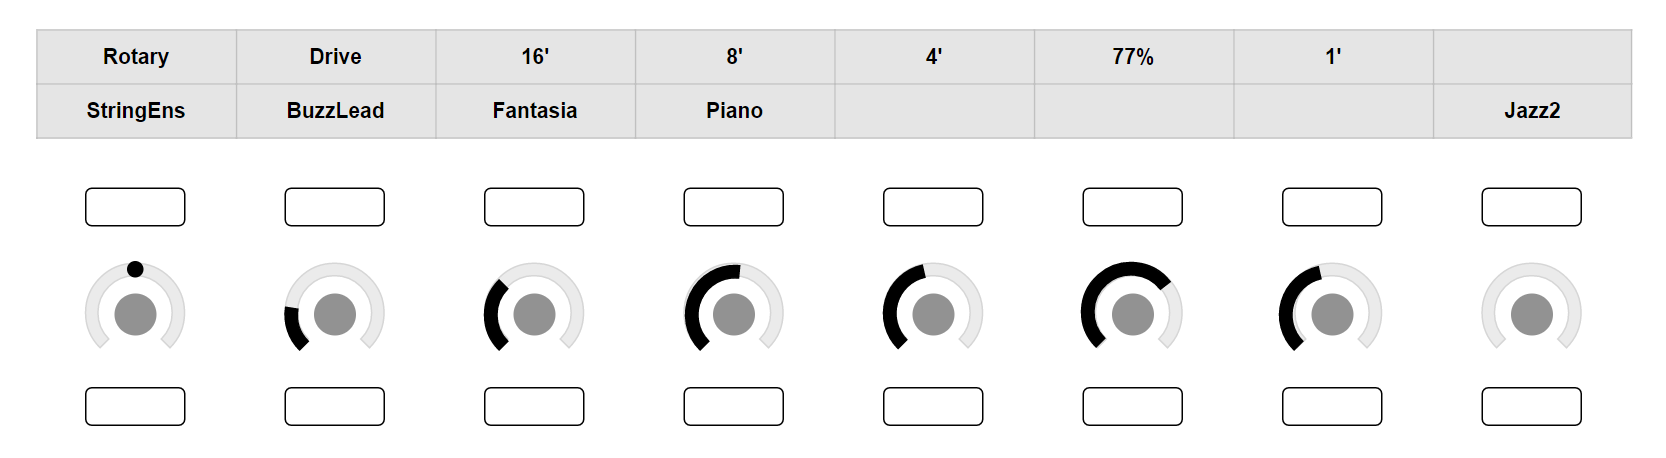
\includegraphics[width=0.9\textwidth]{ControllerUI-PresetDetail}
			\caption{Drátěný model obrazovky \texttt{C2} (ovládání parametrů nástroje)}
			\label{fig:ControllerUI-PresetDetail}
		\end{sidewaysfigure}
		
		\begin{sidewaysfigure}
			\centering
			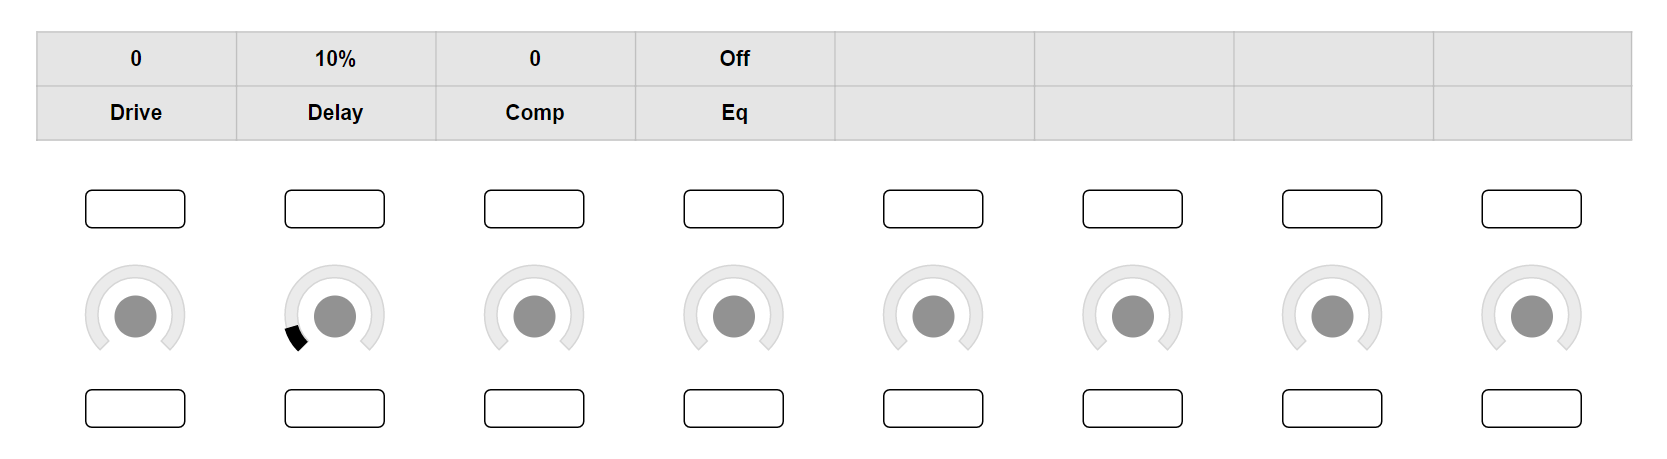
\includegraphics[width=0.9\textwidth]{ControllerUI-EffectOverview}
			\caption{Drátěný model obrazovky \texttt{C3} (souhrnné ovládání efektů)}
			\label{fig:ControllerUI-EffectOverview}			
			\vspace{1.2cm}
			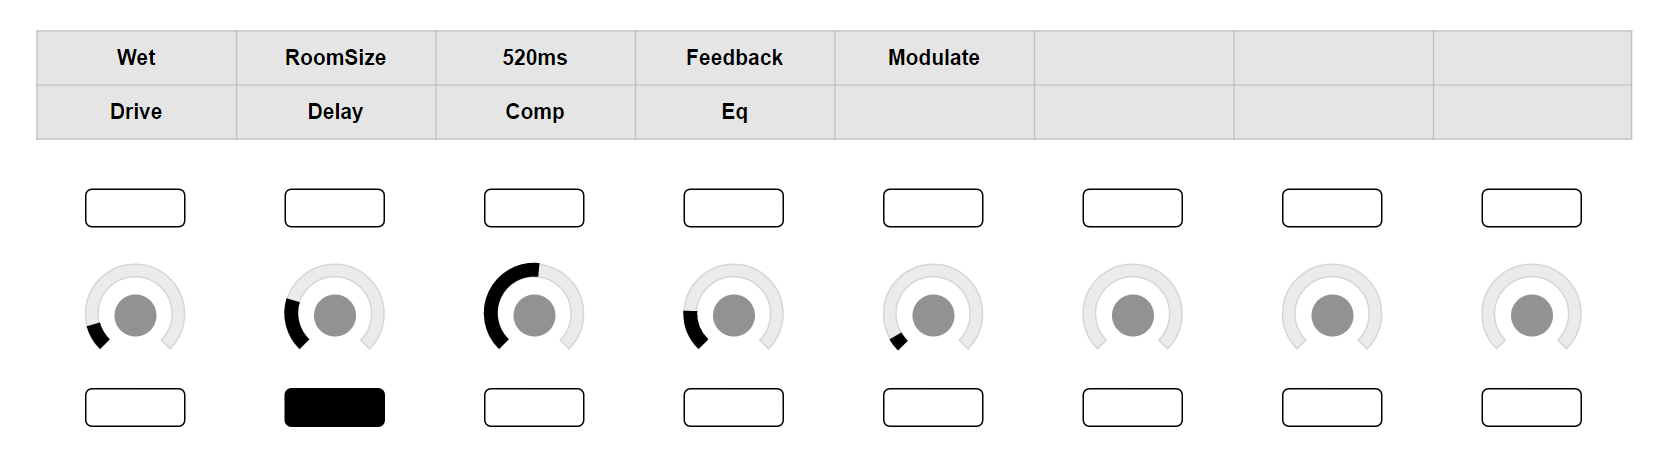
\includegraphics[width=0.9\textwidth]{ControllerUI-EffectDetail}
			\caption{Drátěný model obrazovky \texttt{C4} (ovládání parametrů efektu)}
			\label{fig:ControllerUI-EffectDetail}
		\end{sidewaysfigure}
	
		\subsection{Hlavní navigace}\label{sec:controller-navigation-design}
			Pro hlavní navigaci mezi obrazovkami kontroleru byla zvolena dvojice tlačítek umístěných nalevo od displeje.
			Jednoduchým stisknutím spodního tlačítka dojde k načtení obrazovky ovládání parametrů nástroje.
			Pokud uživatel stiskne vrchní tlačítko, je zobrazena obrazovka procházení presetů.
			Při dvojitém stisknutí jednoho z tlačítek dojde k načtení obrazovky souhrnného ovládání efektů.
			Jestliže bylo dvakrát stisknuto horní z tlačítek, budou zobrazeny vstupní efekty vrstvy, v případě spodního
			tlačítka bude zobrazeno ovládání výstupních efektů pro danou vrstvu.
			Při trojitém stisknutí se dvojice tlačítek chová podobně jako v případě dvojitého stisknutí,
			k ovládání efektů ale nedochází na aktivní vrstvě, ale na globální úrovni.
			Volba aktivní obrazovky je indikována pomocí LED prvku příslušného tlačítka. V případě obrazovek,
			které lze aktivovat vícenásobným stisknutím tlačítka je stav indikován rychlostí blikání LED prvku.			
		
			Pro výběr aktuálního manuálu a vrstvy byla zvolena vertikální řada tlačítek pod dvojicí tlačítek sloužicích k hlavní navigaci.
			Tlačítka představují jednotlivé manuály. Stisknutím tlačítka dojde přepnutí na vrstvu manuálu určené podle počtu stisknutí.
			Aktuální manuál je indikován LED prvkem příslušného tlačítka. Rychlost blikání indikuje pořadí zvolené vrstvy, přičemž
			konstantní rozsvícení LED značí volbu první vrstvy.
		\subsection{Procházení presetů (obrazovka C1)}\label{sec:C1}
			Jak lze vidět z drátěného modelu \ref{fig:ControllerUI-PresetSwitch}, na obrazovce procházení presetů jsou na prvním řádku displeje
			zobrazeny kategorie presetů, na druhém řádku je zobrazen seznam presetů v dané kategorii.
			Jelikož množství presetů v rámci jedné kategorie může být značné, je uplatněno stránkování presetů.
			Pro volbu kategorie a její stránky slouží první řada tlačítek umístěných pod displayem.
			Při stisku tlačítka dojde k volbě příslušné kategorie. Počet stisknutí pak vyjadřuje pořadí stránky presetů, která má být zobrazena.
			
			Na druhém řádku displeje jsou zobrazeny presety pro danou stránku kategorie. Při kliknutí na tlačítko 
			z druhé řady tlačítek pod displayem dojde k výběru aktivního presetu.
			
			Aktuální kategorie a preset jsou indikovány rozsvícenou LED u příslušného tlačítka.
			
			Po aktivování obrazovky je automaticky indikován aktivní preset pro
			aktuální vrstvu a jeho zařazení v kategorii.
			
		\subsection{Ovládání parametrů nástroje (obrazovka C2)}\label{sec:C2}
			Na této obrazovce lze ovládat parametry nástroje a vybrat aktivní preset z historie nedávno aktivovaných presetů (viz diagram \ref{fig:ControllerUI-PresetDetail}).
			V prvním řádku displeje je možné vidět název mapování parametru nástroje nebo jeho aktuální hodnotu. V druhém řádku
			je zobrazena historie nedávno použitých presetů. V posledním poli druhého řádku displeje je pak zobrazen název
			aktuálního presetu.
			
			Aktuální stav hodnoty parametru nástroje je indikován nepřetržitě LED prstencem umístěným okolo otočného enkodéru na základě
			zvolené strategie mapování. Při změně parametru nástroje je hodnota zobrazena i graficky v příslušném poli na displeji, jinak je v poli zobrazen název mapování parametru.
			Formát zobrazení hodnoty parametru na displeji je opět určen strategií mapování parametru.
			
			Při stisku tlačítka z první řady pod displayem dojde k nastavení hodnoty parametru nástroje na výchozí hodnotu určenou aktuálně zvoleným presetem.		
			Pokud uživatel stiskne tlačítko z druhé řady, dojde k načtení presetu příslušného záznamu historie, včetně neuložených rozdílových sad hodnot parametrů nástroje a efektů.
			
		\subsection{Souhrnné ovládání efektů (obrazovka C3)}\label{sec:C3}
			Jelikož efekty většinou disponují jedním hlavním parametrem, který určuje míru použití efektu,
			na obrazovce souhrnného ovládání efektů (viz diagram \ref{fig:ControllerUI-EffectOverview}) lze ovládat pro každý
			efekt právě tento zástupný parametr.
			
			První řádek displeje a související řada tlačítek se chová podobně jako v případě obrazovky ovládání parametrů nástroje
			s tím rozdílem, že jsou použity hlavní mapování parametrů každého efektu namísto mapování parametrů nástroje.
			Navíc je místo zobrazení názvu mapování parametru na displeji vždy zobrazena hodnota parametru, jelikož je zřejmé,
			že je se jedná o hlavní parametr pro daný efekt.
			
			Na druhém řádku displeje je zobrazen seznam dostupných efektů pro danou vrstvu a umístění. Při stisknutí tlačítka
			z druhé řady je načtena obrazovka ovládání všech parametrů příslušného efektu (viz. kapitolu \ref{sec:C4}).
		
		\subsection{Ovládání parametrů efektu (obrazovka C4)}\label{sec:C4}
			Na této obrazovce je k dispozici ovládání parametrů efektu (viz diagram \ref{fig:ControllerUI-EffectDetail}).
			Chování je podobné jako u obrazovky ovládání parametrů nástroje (viz sekci \ref{sec:C2}), druhá řada displeje a tlačítek
			slouží k přepínání ovládaného efektu podobně jako u obrazovky souhrnného ovládání efektů (viz kapitolu \ref{sec:C3}).
		
\chapter{Implementace vlastního řešení}
	\section{Reaktivní programování}
		Pro velkou část aplikace bylo zvoleno reaktivní programovací paradigma, které je orientováno
		na datové toky a šíření změn. Lze tak jednoduše sledovat změny hodnot, provádět 
		nad nimi různé transformace, filtrování, agregaci a další operace. Podporu reaktivního programování přináší do aplikace
		použitý framework RxJS\cite{clow2018observers}. Velkou výhodou je možnost udržování počtu naslouchání
		s využitím např. funkce \\\texttt{switchMap}, zrušení nerelevantních naslouchání pak probíhá automaticky a není předmětem práce programátora.
		Framework RxJS je využitý též knihovnou NGXS zajišťující správu stavu aplikace (viz kapitolu \ref{sec:NGXS}).

	\section{Komunikace přes USB}
		Pro komunikaci s hardwarovým kontrolerem nebylo možné použít dostupné API pro použití MIDI protokolu,
		jelikož se zařízení systému nejeví jako standardní MIDI zařízení. Formát komunikace však příslušné třídě USB rozhraní odpovídá.
		Proto bylo nezbytné implementovat vrstvu, která umožní přijímat a odesílat MIDI zprávy typu CC a SysEx
		podle protokolu USB třídy pro MIDI zařízení\cite{usbmidi}.
		
		Zprávy typu CC jsou opatřeny jednoduchou hlavičkou a celá zpráva má konstantní délku 4B.
		
		SysEx zprávy představují zprávy variabilní délky. Jelikož lze v jednom packetu přenést pouze 4B,
		je třeba zprávy tohoto typu rozdělit na zarovnané části a ty odesílat, resp. zpracovávat samostatně.
		
		Třída \texttt{MidiAdapter} tak poskytuje částečnou implementaci tohoto protokolu. 
		Obsahuje metodu pro odeslání zprávy a možnost naslouchat příchozím zprávám za použití třídy \texttt{Observable} z knihovny RxJS.		
		Třída využívá funkcí třídy \texttt{USBDriver}, jejíž instance je v konstruktora předána s pomocí techniky dependency injection\cite{prasanna2009dependency}.
		
		Třída \texttt{USBDriver} poskytuje jednoduché rozhraní pro komunikaci s připojeným USB zařízením.
		Umožňuje odesílat data a poskytuje možnost naslouchání údalostem typu příjem dat, připojení a odpojení zařízení podobně jako třída \texttt{MidiAdapter}.

	\section{Stavový model aplikace a knihovna NGXS}\label{sec:NGXS}
		Aplikace je rozdělena na klientskou a serverovou část. Jelikož hlavní logika ovládání hardwarového kontroleru a VST host aplikace
		musí vykazovat co nejnižší odezvu, je třeba, aby byl dostupný aktuální stav aplikace v serverové části.
		Zároveň však musí být stav přístupný i části klientské, aby mohly být reflektovány změny stavu iniciované přes
		hardwarový kontroler nebo VST host aplikaci.

		Knihovna NGXS představuje framework pro správu stavu aplikace podle návrhového vzoru Flux\cite{flux}, který vychází ze vzoru CQRS\cite{flux-cqrs}. Výhodou je možnost použití vzoru Observer u celého stavu aplikace a docílit tím asynchronního
		přístupu ke stavu nebo jeho částem\cite{mansilla2018reactive}. Stav je aktualizován tzv. akcemi, které lze kdykoliv vyvolat,
		mají určený jednoznačně identifikovaný typ a mohou nést libovolná data.
		
		Pro synchronizaci stavu mezi klientskou a serverovou částí aplikace byla implementována vrstva, která funguje jako proxy
		pro akce vyvolané v obou částech aplikace. Přenos akcí probíhá přes systém zasílání zpráv poskytovaný frameworkem Electron.
		Veškeré akce vyvolané v jedné z částí aplikace jsou serializovány a odesílány ve formě zprávy do opačné části aplikace, kde
		probíhá deserializace a předání akce ke zpracování frameworkem NGXS. Při vyvolání akce v jedné části aplikace tak dojde
		ke změně stavu v serverové i klientské části zároveň. U každé zprávy lze nastavit příznak určující, že akce nemá být odeslána
		do opačné strany aplikace. Zároveň je možné stanovit tzv. blacklist, tedy seznam akcí, které nebudou předávány druhé straně.
		Lze tak filtrovat např. interní akce frameworku NGXS a jeho přídavných modulů k zamezení vzniku jejich duplicity nebo zacyklení.
		Jelikož obě části aplikace používají pouze část celého stavu, jsou předané akce měnící stav irelevantní pro danou část aplikace  jednoduše ignorovány, jelikož v dané části aplikace není zaregistrována komponenta, která by na zprávy reagovala změnou lokálního stavu.
		Možná je budoucí optimalizace komunikace zamezením přenosu irelevantních akcí.
		
		Při návrhu jednotlivých částí stavu bylo třeba dbát na požadavek, aby nedocházelo k přenosu zpráv (a tedy i vyvolávání automaticky předávaných akcí) s vysokou frekvencí nebo velkým množstvím dat. Ve sdílené části stavu aplikace tak nebude zahrnuta např. informace o aktuálních hodnotách parametrů VST pluginů, jelikož může docházet k jejich intenzivním změnám ze strany VST hosta nebo hardwarového kontroleru.
		
		Struktura modelu stavu aplikace je normalizovaná z důvodu zamezení duplicity dat a zajištění datové konzistence\cite{state-normalization}. Pro CRUD operace nad
		entitami bylo vytvořeno vlastní jednoduché API.
		
		V následujícíh podkapitolách následuje výčet jednotlivých
		částí modelu stavu aplikace.
		
		\subsection{Synchronizace přes IPC}
			Pro klientskou i serverovou část byly implementovány třídy \texttt{IpcActionReceiver} a 
			\texttt{IpcActionTransmitterPlugin}. Třída \texttt{IpcActionTransmitterPlugin} implementuje NGXS API pro tvorbu pluginů a zajišťuje zasílání kopií akcí vyvolaných přes NGXS framework druhé straně aplikace. K příjmu zprávy slouží třída \texttt{IpcActionReceiver}, která akci předá
			NGXS frameworku tak, že simuluje lokální vyvolání dané akce. Zprávy jsou serializovány do formátu JSON a k jejich přenosu dochází
			za použití IPC API frameworku Electron.
		
		\subsection{API pro CRUD operace nad entitami}
			Jelikož skrz celou aplikací bude potřeba provádět nad entitami operace typu přidání, čtení, aktualizaci a odstranění, bylo nejprve implementováno API pro tyto operace, aby nebylo nutné využívat duplicitní
			kód pro každou entitu zvlášť. Implementovány byly operace aktualizace, částečná aktualizace, přidání,
			přidání s případnou aktualizací a odstranění. Operace pro čtení je triviální a každá třída reprezentující
			stav pro danou entitu jí implementuje zvlášť.						
		
		\subsection{LayoutState}
			V tomto stavu budou obsažené informace o uložených projektech VST host programu Bidule.
			Model používá API pro CRUD operace. Stav je globální, jeho obsah tedy není ukládán
			v závislosti na právě otevřeném projektu. Kromě samotných entit obsahuje informace o 
			právě načteném projektu a příznak určující zda právě probíhá načítání layoutu.
			V modelu je obsažena logika pro řazení projektů podle času posledního použití.			
			
		\subsection{FrontendState}
			Tento stav je jediný, který není sdílený mezi serverovou a klientskou částí.
			Obsahuje informace typické pro klientskou část, např. zda již byla aplikace inicializována.
			Původním záměrem bylo zahrnout i informace o navigaci, ale k tomuto
			účelu byla později vybrána knihovna \texttt{ngxs/router-plugin}, která tuto informaci
			obsahuje v rámci svého vlastního stavu a poskytuje též možnost provést změnu navigace
			odesláním tzv. akce za použití frameworku NGXS.
		
		\subsection{VSTState}
			V tomto stavu jsou obsaženy informace o dostupných VST pluginech. Stav je uložen 
			pro každý projekt zvlášť (viz. kapitolu TODO) a je sdílený klientskou i serverovou částí aplikace.
			Model používá z API pro CRUD operace pouze funkce pro přidání a aktualizaci.
			Pro získávání entit představujících virtuální nástroje a efekty jsou přítomné příslušné metody.
			Zároveň je zde implementována obsluha akcí pro správu stránek mapování parametrů
			VST pluginů pro virtuální nástroje i efekty.
					
		\subsection{ManualState}
			Tento stav obsahuje informace o manuálech a vrstvách dostupných v otevřeném projektu a je sdílený klientskou i serverovou částí aplikace. Není ukládán do perzistentního úložiště.
			Model používá z API pro CRUD operace pouze funkce pro přidání, jelikož k načtené stavu
			dochází pouze při otevření projektu. Obahuje informaci o aktuálně zvolené vrstvě, model obsahuje metodu
			pro získání aktuálně zvoleného manuálu.
		
		\subsection{SessionState}
			V tomto stavu jsou uloženy informace o aktuálním sezení. Stav je sdílený klientskou i serverovou částí aplikace a není ukládán do perzistentního úložiště.
			Mezi obsažené informace patří např. ID aktuálně zvolené vrstvy a další informace vycházející z aktuálního stavu navigace z pohledu celé aplikace.
			
		\subsection{ParamMappingPageState}
			Stránka mapování může obsahovat až 8 jednotlivých mapování, v systému se s ní pracuje dále jako s elementárním celkem. 
			Ve stavu \\\texttt{ParamMappingPageState} je pak uložna aktuálně načtená stránka mapování. Stav není ukládán do perzistentního úložiště a je sdílen klientskou i serverovou částí aplikace. 
			Kromě funkcí API pro CRUD operace obsahuje model i logiku pro správu jednotlivých mapování. 
			Poskytuje také možnost řazení jednotlivých mapování v rámci stránky a informaci
			o aktuálním zvoleném mapování. Impelementována je zde i logika pro načítání uložených stránek mapování
			z VST efektů a nástrojů.
			
		\subsection{PresetCategoryState}
			Tento stav obsahuje uložené kategorie presetů. Je sdílen klientskou a serverovou částí aplikace
			a jeho obsah je ukládán do perzistentního úložiště pro každý projekt zvlášť.
			Používá API pro CRUD operace obsahuje. Dále poskytuje logiku vyřizování CRUD operací samotných presetů
			z pohledu kategorie. Lze tak presety v rámci kategorie řadit, přidávat, duplikovat, či odebírat.
			
		\subsection{PresetState}
			V tomto stavu jsou obsažené informace o uložených presetech. Je sdílen klientskou a serverovou částí aplikace a jeho obsah je ukládán do perzistentního úložiště pro každý projekt zvlášť.
			Kromě funkcí z API pro CRUD operace obsahuje logiku pro duplikaci presetů vč. generování
			názvu duplikovaných presetů.
			
		\subsection{PresetSessionState}
			Tento stav pro každou vrstvu zvlášť uchovává informace o aktuálně načteném presetu.
			Mezi tyto informace patří např. historie naposledy použitých presetů a příznaky pro 
			ovládání úpravy aktuálního presetu. V modelu stavu je obsažena logika pro správu historie naposledy použitých presetů.
			Stav je sdílen mezi klientskou a serverovou částí aplikace a není ukládán do perzistentního úložistě.
		
	\section{OSC a VST host Bidule}
		
		Pro obousměrnou komunikaci serverové části vlastní aplikace s VST hostitelskou aplikací přes protokoly UDP a OSC je použita knihovna \texttt{node-osc}.
		Tato knihovna umožňuje odesílat a přijímat OSC zprávy asynchronním způsobem. Příjem zpráv lze realizovat 
		nasloucháním zprávám odpovídajícím zadanému vzoru. Pokud již daný příjem zpráv není relevantní, je třeba naslouchání zastavit,
		aby nedocházelo ke zbytečnému čerpání systémových prostředků. Proto byla zavedena třída \texttt{OscService}, která 
		umožňuje vytvořit k naslouchání instanci třídy \texttt{Observable} z frameworku RxJS. Třída též obsahuje 
		mapu posledních hodnot pro danou OSC adresu. Lze tak použít i přístup \texttt{BehaviorSubject} z frameworku RxJS,
		kdy lze naslouchat změnám hodnot, po inicializaci naslouchání je však odeslána úvodní hodnota.
		
		\subsection{Načítání projektů}
		Program Bidule umožňuje načtení projektu ze zvoleného XML souboru odesláním OSC zprávy. Tímto způsobem
		je ve vlastní aplikaci implementováno načítání projektů. Při otevření projektu dojde k odeslání příslušné
		OSC zprávy do programu Bidule. Dále se v časovém intervalu 1s odesílá tzv. beacon zpráva vyžadující odpověď.
		Pokud odpověď dorazí, znamená to, že je projekt již načtený. Pokud odpověď nedorazí, znamená to, že se projekt stále v programu Bidule načítá,	nebo že došlo k chybě. Při zavření projektu dojde v programu Bidule k načtení dodaného prázdného projektu.
	
		\subsection{Parametry modulů}
		V programu Bidule může představovat modul buďto některý z interních modulů nebo VST plugin. Každý modul poskytuje seznam svých vlastních parametrů.
		Program Bidule pro tyto parametry umožňuje jejich hodnoty měnit a naslouchat jejich změnám s pomocí protokolu OSC.
		Zároveň pro každý modul zavádí obecné parametry, jako např. pracovní mód, pořadí vybraného presetu apod.
		Číselné hodnoty parametrů jsou normalizovány na hodnotu 1.

		\subsection{Zobrazení UI modulu}
		Přes protokol OSC lze v programu Bidule též zobrazit nebo schovat uživatelské rozhraní jakéhokoliv modulu a zpracovávat notifikace
		o jeho zobrazení, resp. skrytí uživatelem. Ve vlastní aplikaci nejsou notifikace zpracovávány. Zobrazení uživatelského rozhraní modulu
		probíhá na žádost uživatele nebo při editaci konfigurace za použití tzv. funkce learn, kdy se konfigurace mění v závislosti
		na akcích provedených přímo v prostředí modulu programu Bidule.

		\subsection{Ovládání pracovního módu modulů}
		V programu Bidule každý modul poskytuje obecný parametr představující svůj aktuální pracovní mód. Ten může nabývat následujících hodnot:
		\begin{itemize}
			\item \texttt{Processing} - modul je aktivní a zpracovává data.
			\item \texttt{Bypass} - modul je aktivní a jsou do něj odesílána data, výstupní data jsou však ignorvána.
			\item \texttt{Mute} - modul není aktivní a nevyužívá výpočetní výkon systému.
		\end{itemize}
		Jelikož je jedním z požadavků na systém optimalizace využití systémových prostředků, je třeba ovládat
		pracovní mód modulu dynamicky. Děje se tak u modulů představujících VSTi pluginy, pro danou vrstvu 
		tak může být současně aktivní pouze jeden virtuální hudební nástroj. V budoucnu je možné použít ovládání pracovního módu
		i pro efekty podle předem zadaných pravidel pro hlavní mapování parametrů efektu k docílení další optimalizace
		systémových prostředků.

		\subsection{Volba presetů VST pluginů}
		Pro každý modul program Bidule zavádí obecné parametry představující číslo a název aktuálního zvoleného presetu.
		Tyto parametry jsou použité u jedné ze strategií inicializace presetu v rámci tzv. funkce learn, kdy dochází
		ke změnám konfigurace v prostředí programu Bidule, a v rámci samotné inicializace presetu.

		\subsection{Synchronizace vlastních parametrů modulů}
		Přes protokol OSC lze také ovládat všechny vlastní parametry modulů v projektu programu Bidule.
		K nastavení hodnot dochází při ovládání hardwarovým kontrolerem a inicializaci presetu.
		Naslouchání změnám hodnot se využívá při prezentaci hodnot na hardwarovém kontroleru
		a při aktivní tzv. learn funkci, kdy dochází ke změně konfigurace mapování parametrů v prostředí programu Bidule.

		\subsection{Generování MIDI zpráv}
		Jelikož je jednou ze strategií inicializace virtuálního nástroje odeslání MIDI zprávy typu program change,
		byl do architektury projektu programu Bidule zahrnutý vlastní modul, který umožňuje přes OSC odeslat požadovanou MIDI zprávu
		do libovolného virtuálního nástroje. Tento modul bude použitý také u vyslání obecných MIDI zpráv,
		mezi které patří např. zprávy typu panic, které zajistí přerušení všech znějících tónů.
	
	\section{Automap a hardwarový kontroler}\label{sec:automap-hw-controller}
		Pro podporu komunikace s hardwarovým kontrolerem přes protokol Automap byla vytvřena speciální vrstva.
		V budoucnu je možno tuto vrstvu nahradit jinými implementacemi pro podporu dalších ovládacích zařízení.
		Vrstva vužívá třídu \texttt{MidiAdapter} pro přenos zpráv podle protokolu Automap.
		V následujících podkapitolách jsou popsány jednotlivé části této vrstvy, která zajišťuje
		vstupně-výstupní operace s připojeným hardwarovým kontrolerem. 

		\subsection{Inicializace zařízení}
		Po připojení zařízení protokol Automap přikazuje provést tzv. handshake, tedy výměnu zpráv
		pro zahájení komunikace. Po připojení hardwarového kontroleru dojde k automatickému odeslání zprávy do zařízení
		a systém čeká na příjem potvrzující zprávy. 
		Obě zprávy jsou typu SysEx a nesou informaci o verzi protokolu a další konfiguraci zařízení.
		
		\subsection{Tlačítka kontroleru}
		Protokol Automap umožňuje přes MIDI zprávy typu CC předávat informace o stisknutí tlačítka
		hardwarového kontroleru. Zároveň poskytuje možnost nastavit stav LED podsvícení příslušného tlačítka.
		Jelikož v samotném hardwarovém kontroleru není k dispozici žádná další logika, bylo potřeba
		implementovat rozšířenou logiku chování tlačítek v aplikaci.
		
		Samotná tlačítka uživatelského rozhraní kontroleru lze rozdělit do logických celků.
		Pro reprezentaci takového celku v kódu vznikla třída \texttt{ButtonGroup}. Tato třída
		obsahuje metody pro nastavení stavu jednotlivých LED a všech LED v rámci celku.
		Zároveň za použití třídy \texttt{EventEmitter}, která implementuje rozhraní \texttt{Observable} 
		z frameworku RxJS, poskytuje možnost naslouchání na událost stisku tlačítka reprezentované třídou \texttt{ButtonClickEvent}.
		Tlačítka jsou identifikována číslem stanoveným protokolem Automap, které je při komunikaci přenášeno
		v MIDI zprávě typu CC. Třída \texttt{ButtonGroup} v konstruktoru přijímá seznam identifikátorů tlačítek
		v daném celku. Zároveň poskytuje i možnost nastavení příznaku pro ignorování stisknutí.
		Tento příznak lze zadat pro jednotlivá tlačítka zvlášť nebo hromadně pro všechna tlačítka v rámci skupiny.
		Pokud je stisknuto tlačítko, které nemá nastavený příznak ignorování stisku, dojde zároveň k jeho podsvícení dokud není tlačítko uvolněno.
		
		Pro instanci třídy typu \texttt{ButtonGroup} lze též nastavit objekt impelmentující rozhraní \texttt{ClickHandlerInterface}, který reaguje
		na stisknutí, resp. uvolnění tlačítka. Nastavení lze provést globálně pro celou skupinu tlačítek nebo pro každé tlačítko zvlášť.
		Rozhraní \texttt{ClickHandlerInterface} umožňuje třídě vyvolat vlastní událost představující stisknutí tlačítka.
		Vlastní událost musí splňovat rozhraní třídy \texttt{ButtonClickEvent}. Pro zpracování vstupu definuje rozhraní metody,	které jsou zavolány po stisknutí, nebo uvolnění tlačítka.
		Jako výchozí implementace rozhraní \texttt{ClickHandlerInterface} je při vytváření třídy \texttt{ButtonGroup} inicializována instance třídy 
		\texttt{SimpleClickHandler}, která zanedbává informace o uvolnění tlačítka a vyvolává událost představující stisknutí tlačítka 
		ihned po fyzickém stisknutí tlačítka. 
		Další implementací rozhraní \texttt{ClickHandlerInterface} je třída \texttt{MultiClickHandler}, která zajišťuje zpracování vícenásobného stisknutí tlačítka. 
		V rámci instance lze nastavit nejvyšší počet stisknutí tlačítka a maximální časový rozestup mezi jednotlivými stisky tlačítka, než dojde k vyvolání události stisknutí tlačítka. 
		Událost \\\texttt{ButtonMultiClickEvent} poté nese kromě identifikátoru stisknutého tlačítka i informaci o počtu stisknutí tlačítka.
		V budoucnu je možné implementovat např. třídu pro zpracování podržení tlačítka, kde budou zohledněny i vstupní události fyzického uvolnění tlačítka.
		
		Jelikož mají logické celky tlačítek často pravoúhlý tvar, kde je výhodné použít adresaci pomocí
		kartézské soustavy souřadnic, byla pro tento účel implementována třída \texttt{ButtonMatrix} využívající
		s pomocí kompozice třídu \texttt{ButtonGroup}. V konstruktoru je navíc vyžadována informace o rozměrech mřížky a identifikátor prvního tlačítka. 
		Identifikátory dalších tlačítek jsou vypočítány automaticky podle číslování plynoucího z protokolu Automap.
		Události stisknutí tlačítka v mřížce, kterým lze naslouchat, obsahují informaci o souřadnicích tlačítka. Reprezentuje je třída \texttt{ButtonMatrixEvent},
		jejíž rozhraní vychází z třídy \texttt{ButtonClickEvent}. K dispozici je i vazba na původní událost typu \texttt{ButtonClickEvent}, která je řešena pomocí kompozice.
		
		Pro podporu přerušovaného podsvícení tlačítek byla zavedena třída \\\texttt{InterruptionClock}. Díky této třídě lze 
		udržovat přerušované podsvícení synchronní napříč celou aplikací. Třída podporuje čtyři stupně rychlosti blikání.
		S pomocí třídy \texttt{EventEmitter} z frameworku RxJS lze naslouchat obdélníkovému signálu představujícímu stav podsvícení podle zvoleného stupně frekvence přerušení.

		\subsection{Displej kontroleru}
		Příkazy pro ovládání displeje využívají MIDI zpráv typu SysEx. Je možné smazat celý obsah displeje a 
		vypsat ASCII řetězec na pozici určené dvojicí souřadnice. API třídy \texttt{Display} pro ovládání displeje tyto funkce poskytuje.
		Tato vrstva též zajišťuje možnost vypsat text do příslušné buňky s automatickým zarovnáním, nebo zkrácením řetězců.
		Veškeré operace lze provést okamžitě, nebo je provádět pouze lokálně a poté odeslat do zařízení celý obsah displeje.
		Pro tuto optimalizace třída zahrnuje buffer obsahující aktuální obsah celého displeje.

		\subsection{Rotační enkodéry kontroleru}
		Hardwarový kontroler poskytuje tři druhy otočných ovladačů. Tzv. nekonečné knoby (rotační enkodéry obklopené
		prstencem LED), standardní potenciometry a rotační enkodér bez prstence LED pro hlavní navigaci.
		Všechny otočné ovladače podporují vyslaní signálu při dotyku, resp. jeho přerušení. 
		
		U nekonečných knobů lze nastavit mód zobrazení hodnoty na LED prstenci (např. zobrazení bodem, kruhovou výsečí).
		Při otočení zařízení odešle MIDI zprávu určující směr a rychlost pohybu.
		
		Rotační enkodér pro	hlavní navigaci lze stisknout a odeslat tak příslušnou MIDI zprávu. Při jeho otočení
		zařízení odešle MIDI zprávu podobně jako u rotačních enkodérů s LED prstencem.
		
		U klasických potencimetrů zařízení odesílá při změně hodnoty aktuální hodnotu vyjádřenou 7b.
		
		Třída \texttt{Knobs} zastupuje skupinu nekonečných knobů s LED prstencem. Umožňuje pro každý knob změnit mód zobrazení hodnoty a
		nastavit hodnotu indikovanou LED prstencem. Též poskytuje s pomocí třídy \texttt{EventEmitter} z frameworku RxJS události, kterým lze naslouchat.
		Třída \texttt{KnobEvent} představuje rodičovskou třídu pro všechny události knobů. Třída \texttt{RotationKnobEvent} jí dědí a přidává informaci
		o směru a rychlosti otočení. Naslouchat lze událostem dotyku, uvolnení dotyku a otočení.
		
		\subsection{Architektura}
		Třídy implementující jednotlivé části vrstvy jsou použity ve větších celcích určených rozmístením prvků na hardwarovém kontroleru.
		Např. třída \linebreak	\texttt{NavigationRegionDriver}, která představuje množinu ovládacích prvků určených k navigaci, využívá dvě instance třídy \texttt{ButtonGroup}.
		Třída \texttt{DisplayRegionDriver} pro ovládní prvků v oblasti displeje obsahuje instance tříd \texttt{Display}, \texttt{Knobs} a \texttt{ButtonMatrix}.
		Tyto celky jsou použity v implementaci logiky uživatelského rozhraní hardwarového kontroleru.
		
	\section{Uživatelské rozhraní hardwarového kontroleru}
		Jednotlivé části vrstvy uživatelského rozhraní hardwarového kontroleru jsou orchestrovány s pomocí třídy \texttt{KeyboardRouter}.
		Ta zároveň slouží pro navigaci v rámci uživatelského rozhraní kontroleru. Pro tento účel poskytuje metodu \texttt{navigate}, která
		způsobí načtení požadovaného stavu navigace. Stav navigace je vyjádřen řetězcem, jednotlivé stavy nemůžou obsahovat žádná metadata. Ta je případně
		vhoné přenášet ve vlastnosti \texttt{KeyboardRoute} stavu \texttt{SessionState} s využitím knihovny NGXS. Třída \\\texttt{KeyboardRouter} obsahuje referenci na všechny komponenty řídící jednotlivé 
		části uživatelského rozhraní hardwarového kontroleru. Podle aktuálního stavu navigace určuje, které komponenty jsou právě aktivní. 
		Každá komponenta pro řízení části uživatelského rozhraní kontroleru musí implementovat rozhraní \texttt{MortalInterface}, které obsahuje deklaraci metody \\\texttt{onInit} a \\\texttt{onDestroy}.
		Z pohledu návrhového vzoru MVC\cite{reenskaug1979original} se chovají takové komponenty dohromady jako view a controller. V následujících podkapitolách
		budou diskutovány jednotlivé komponenty pro řízení části uživatelského rozhraní.
		
		\subsection{Komponenty pro ovlání oblasti displeje}\label{sec:display-area-components}
			Jelikož lze na displeji dobře indikovat aktuální chování přidružených prvků, oblast displeje může být použita pro větší množství obrazovek.
			V této podkapitole budou diskutovány komponenty pro řízení oblasti displeje. Všechny komponenty pracují s vrstvou poskytující vstupně-výstupní operace s připojeným hardwarovým kontrolerem (viz kapitolu \ref{sec:automap-hw-controller}). Využívají pouze část vrstvy, která poskytuje ovládání prvků oblasti displeje, tedy třídu \texttt{DisplayRegionDriver}.
					
			\subsubsection{Třída ParamMappingContoller}
				Tato komponenta ovládá pouze jeden řádek oblasti displeje a měla by být tedy použita v rámci komponenty představující celou obrazovku.
				Je využitá v třídách \texttt{InstrumentDetailController}, \texttt{EffectOverviewController} a \texttt{EffectDetailController} implementující obrazovky C2 - C4 (viz kapitoly \ref{sec:C2}, \ref{sec:C3}, \ref{sec:C4}). Zajišťuje chování pro ovládání a indikaci parametrů VST pluginů. Aktuálně ovládané parametry a jejich mapování načítá ze stavu \texttt{ParamMappingPageState}.
				U otočných enkodérů nastavuje mód zobrazení hodnoty na LED prstencích okolo otočných enkodérů a indikuje hodnotu na LED prstenci podle strategie mapování. Též
				reaguje na události otočného enkoderu. Při jeho otočení podle strategie mapování vyvolá akci aktualizace hodnoty parametru VST pluginu.
				Zobrazení na displeji poskytuje standardně název ovládaného parametru, pokud však není nastavený příznak pro trvalé 
				zobrazení hodnot.
				Aktuální hodnota ovládaného parametru je zobrazena jen pokud dojde k její změně nebo pokud se uživatel dotkne příslušného otočného enkoderu.
				Formát zobrazení hodnoty na displeji je určen stragetií mapování.
				Hodnota parametru je zobrazena jen po určitý čas, poté se opět zobrazení vrátí na název ovládaného parametru. 
				Toto chování je zajištěno netriviální logikou vyjádřenou za použití reaktivního programování a knihovny RxJS.

			\subsection{ParamMappingLoaderService}
				Třída \texttt{ParamMappingLoaderService} zajišťuje automatickou aktualizaci stavu \texttt{ParamMappingPageState} při změně aktuální vrstvy nebo presetu.
				Pokud je zvolena vrstva i preset, načte stránku mapování parametrů nástroje danou v presetu, jinak načte prázdnou stránku mapování.
				
			\subsection{Třída LastPresetsController}
				Podobně jako u třídy \texttt{ParamMappingController} je ovládán pouze jeden řádek oblasti displeje. Na řádku jsou zobrazeny
				záznamy historie posledních použitých presetů a aktuální preset. Při stisknutí příslušného tlačítka dojde k vyvolání 
				akce \texttt{SelectPresetAction} určující, který preset má být aktuálně načten. Třída načítá data ze stavu \texttt{PresetSessionState}
				pomocí metody \texttt{getCurrentHistory}, jejíž výstup je závislý na aktuální vrstvě. Při změně aktivní vrstvy tedy dojde
				k zobrazení záznamů historie pro danou vrstvu.
							
			\subsection{Třída EffectSwitchController}
				Pro přepínání ovládaných efektů byla vytvořena třída \texttt{EffectSwitchController}. 
				Ovládá pouze jeden řádek oblasti displeje a je používaná třídami \texttt{EffectOverviewController} a \texttt{EffectDetailController}. Data načítá ze stavů \texttt{SessionState}, \texttt{ManualState} a \texttt{VstState}.
				Poskytuje uživateli seznam efektů dostupných pro aktuálně zvolený kontext, který zahrnuje aktuální vrstvu a konfiguraci
				zobrazení efektů, tedy umístění efektů (vstup nebo výstup) a příznak pro ovládání globálních efektů.
				Při stisknutí tlačítka dojde k vyvolání vlastní události volby efektu s použitím třídy \texttt{EventEmitter} z frameworku RxJS. Aktivní efekt je možné nastavit s použití metody \texttt{SetActiveEffect}, která interně využívá
				třídu \texttt{BehaviorSubject} z frameworku RxJS.			
							
			\subsubsection{Třída InstrumentDetailController}
				Tato třída vužívá v kombinaci tříd \texttt{ParamMappingController} a \texttt{LastPresetsController} tak, aby bylo dosaženo kýženého chování (viz kapitolu \ref{sec:C2}).
				Aktualizace stránky mapování parametrů nástroje je implementována ve třídě \texttt{ParamMappingLoaderService}.
				
			\subsubsection{Třída EffectOverviewController}
				Obrazovka souhrnného ovládání efektů (viz kapitolu \ref{sec:C3}) je implementována třídou \texttt{EffectOverviewController},
				která využívá jako podkomponenty třídy \texttt{EffectSwitchController} a \texttt{ParamMappingContoller}.
				Pokud je vyvolána událost volby efektu instancí třídy \texttt{EffectSwitchController}, dojde k nastavení příslušného stavu navigace v rámci hardwarového kontroleru a je načtena obrazovka detailu efektu (viz kapitolu \ref{sec:C4}).
				U instance třídy \texttt{ParamMappingController} je nastaven příznak pro trvalé zobrazení hodnoty parametru efektu.
				Aktualizace stránky mapování parametrů probíhá automaticky při změně konfigurace dostupných efektů vyvoláním akce \texttt{LoadParamMappingPageAction}. U každého dostupného efektu je vybráno hlavní mapování a z těchto mapování
				je poté sestrojena výsledná stránka mapování. 			
				
			\subsection{Třída EffectDetailController}
				Podobně jako u třídy \texttt{EffectOverviewController} je u této třídy využita komponenta \texttt{EffectSwitchController},
				s pomocí které je též indikován stav aktuálně ovládaného efektu. Událost volby efektu je buď 
				reflektována změnou stavu určením nového aktivního efektu, nebo je uživatel přesměrován na obrazovku souhrnného ovládání efektů (viz kapitolu \ref{sec:C3}).
				Zároveň je třídou \texttt{EffectDetailController} využita i komponenta \texttt{EffectOverviewController} poskytující
				stránku mapování určenou aktuálně ovládaným efektem. Při změně části stavu určující aktuálně ovládaný efekt
				je vyvolána akce načtení stránky mapování parametrů z daného efektu.
		
			\subsection{Třída PresetController}
				Třída PresetController představuje implementaci obrazovky C1 (viz kapitolu \ref{sec:C1}). 
				Zajišťuje procházení kategorií presetů a volbu a indikaci aktuálního presetu.
				Data získává prostřednictvím stavů \texttt{SessionState}, \texttt{PresetCategoryState}, \texttt{PresetState} a \texttt{PresetSessionState}.
				Aktuální zvolená kategorie je obousměrně synchronizována s desktopovým uživatelským rozhraním aplikace.
				Pro možnost stránkování je využitá třída pro zpracování vícenásobného stisku tlačítka \texttt{MultiClickHandler}.
				Netriviální logika je implementována za použití reaktivního programování ve frameworku RxJS.
		
			\subsubsection{Třída EmptyController}
				Instance této komponenty je načtena po spuštění aplikace nebo připojení hardwarového kontroleru k systému. Nereaguje na žádné vstupy od uživatele, na displeji zobrazí informativní hlášku.
						
		
		\subsection{Ostatní komponenty}
			\subsubsection{Třída LayerController}
				Třída \texttt{LayerController} implementuje chování čtveřice tlačítek nalevo pod displejem. Slouží k určování a indikaci aktuálně zvoleného manuálu a vrstvy.
				Tlačítka představují jednotlivé manuály. Rychlost blikání tlačítek značí pořadí vrstvy s využitím třídy \\\texttt{InterruptionClock}. Pro nastavení
				aktuálního manuálu a vrstvy je využita třída pro zpracování událostí stisknutí tlačítka \\\texttt{MultiClickHandler}.
				V případech, kdy kvůli omezením není možné přepínat aktuální vrstvu (např. při editaci presetu) je potlačeno veškeré ovládání a indikace aktuální vrstvy.
				Komponenta je globální a její instance je tedy aktivní po celou dobu běhu aplikace.
			
			\subsubsection{Třída DisplayModeController}
				K přepínání obrazovek, tedy určení aktivní komponenty ovládající oblast displeje, slouží třída \texttt{DisplayModeController}. Dvojicí tlačítek
				umístěných nalevo od displeje lze zobrazit až 6 možných obrazovek (viz kapitolu \ref{sec:display-area-components}). Chování tlačítek využívá
				tříd \texttt{MultiClickHandler} a \texttt{InterruptionClock} tak, aby splnily požadované chování (viz kapitolu \ref{sec:controller-navigation-design}).
	
	\section{Desktopové uživatelské rozhraní}
		Pro desktopové uživatelské rozhraní byl zvolen framework Angular Material, který přináší běžné prvky
		uživatelského rozhraní pro jejich použití ve frameworku Angular. Aplikace vužívá prvky pro rozvržení
		částí UI, formuláře, tlačítka, seznamy a další. Stav desktopového uživatelského rozhraní je do značné míry
		nezávislý na stavu uživatelského rozhraní hardwarového kontroleru. Výjimky budou popsány v následujících podkapitolách, které 
		popisují jednotlivé části desktopového uživatelského rozhraní.
		
		\subsection{Rozdělení do modulů}
			Podle doporučeného návrhu architektury je desktopová část aplikace rozdělena do modulů, které řeší jednotlivé části problémové domény\cite{ng-modules}.
			V rámci modulu lze např. určit konfiguraci pro lokální navigaci, zavádět znovupoužitelné komponenty a implementovat vlastní direktivy pro šablony.
			Kromě kořenového modulu \texttt{AppModule} aplikace obsahuje následující klíčové moduly:
			\begin{itemize}
				\item \texttt{HomeModule}
				\item \texttt{MaterialModule}
				\item \texttt{SharedModule}
				\item \texttt{ParamMappingModule}
				\item \texttt{VstModule}
				\item \texttt{LayoutModule}
				\item \texttt{InstrumentModule}
				\item \texttt{EffectModule}
				\item \texttt{PresetModule}
			\end{itemize}
		
		\subsection{Navigace}
			Pro účely navigace v rámci desktopového uživatelského rozhraní využívá aplikace nativního přístupu poskytovaného
			frameworkem Angular (s využitím modulu \texttt{RouterModule}).
			Knihovna \texttt{@ngxs/router-plugin} pak zajišťuje synchronizaci aktuálního stavu navigace s částí stavu v rámci knihovny NGXS.
			
			V modulu \texttt{AppRoutingModule} pro zajištění hlavní navigace v rámci kořenového modulu jsou definovány následující stavy navigace identifikované prefixem cesty ve formě řetězce. Jednotlivé moduly pak řeší svojí lokální navigaci zvlášť.
			\begin{itemize}
				\item \texttt{''} - modul \texttt{HomeModule} pro zobrazení úvodní obrazovky
				\item \texttt{'layouts'} - modul \texttt{LayoutModule} zajišťující správu uložených projektů programu Bidule
				\item \texttt{'instruments'} - modul \texttt{InstrumentModule} pro práci s virtuálními hudebními nástroji
				\item \texttt{'effects'} - modul \texttt{EffectModule} pro práci s virtuálními efekty
				\item \texttt{'presets'} - modul \texttt{PresetModule} pro správu uložených presetů
				\item \texttt{'**'} - tzv. fallback, který zajistí zobrazení chybové obrazovky pro neplatné cesty navigace.
			\end{itemize}		
		
			Jednotlivé stavy navigace mohou být aktivovány pouze za určitých omezení, např. pokud je načtený projekt programu Bidule. 
			Omezení jsou vyjádřena tzv. guardy, které představují např. třídy \texttt{NoLayoutGuard} a \texttt{LayoutGuard} z modulu \texttt{LayoutModule}.
			
			Ke změně stavu navigace uživatelem slouží vertikální menu definované globálně v rámci hlavní komponenty \texttt{AppComponent} z modulu \texttt{AppModule}. Pro vykreslené menu je použita komponenta \texttt{MatSidenav} z frameworku Angular Material.
			
			Navigace v rámci uživatelského rozhraní harwdarového kontroleru je do značné míry nezávislá na stavu navigace desktopového uživatelského rozhraní aplikace.
			Výjimkou je případ editace některých částí konfigurace projektu, kdy v rámci uživatelského rozhraní hardwarového kontroleru dochází k nastavení stavu navigace a odepření možnosti jeho změny.
			
		\subsection{HomeModule}
			V tomto modulu se nachází implementace komponenty pro zobrazení úvodní obrazovky aplikace. Komponenta \texttt{HomeComponent}
			neobsahuje žádnou logiku, obsažená je pouze jednoduchá šablona. Obrazovka je načtena pouze po inicializaci aplikace.
			
		\subsection{MaterialModule}
			Tento jednoduchý modul je importován všemi moduly, které pracují s knihovnou Angular Material.
			Exportuje veškeré prvky knihovny Angular Material, které jsou použity napříč celou aplikací.
			
		\subsection{SharedModule}
			V modulu \texttt{SharedModule} jsou implementovány veškeré komponenty, které mohou být použity napříč celou aplikací.
			Obsahuje např. komponentu pro zobrazení chybového stavu, obecný dialog pro zadání jména (třída \texttt{NamedEntityDialogComponent}) a direktivu pro potvrzení libovolné akce uživatelem (třída \texttt{ConfirmationDirective}).
			
		\subsection{ParamMappingModule}
			Tento modul poskytuje znovupoužitelnou komponentu \texttt{ParamMappingPageComponent} pro správu stránek mapování parametrů VST pluginů. Ta umožňuje přidávat, odebírat a upravovat jednotlivé položky stránky mapování. Pro zadávání názvu položky
			využívá komponentu \texttt{NamedEntityDialogomponent} definovanou v modulu \texttt{SharedModule}.			
			Pro každou položku umožňuje zvolit strategii mapování. Rozhraní \texttt{AbstractParamMappingStrategyComponent} představuje API pro komponenty umožňující konfiguraci konkrétního mapování. Díky této abstrakci lze v budoucnu přidávat jednoduše další 
			strategie, aniž by bylo potřeba upravovat již existující kód. Návrh tedy splňuje charakteristiky OCP\cite{ocp}.
			
			Třída \texttt{LinearParamMappingStrategyComponent} implementující rozhraní \texttt{AbstractParamMappingStrategyComponent}
			umožňuje konfigurovat lineární strategii mapování parametrů VST pluginů. Využívá formulářových prvků pro zadávání
			hodnot konfigurace. Přináší pro uživatele též možnost využití tzv. learn metody, kdy dochází ke změnám v konfiguraci
			přímo z prostředí VST pluginu v programu Bidule. S využitím této metody lze zadávat minimální a maximální hodnotu
			parametru VST pluginu.		
		
		\subsection{VstModule}
			Modul \texttt{VstModule} obsahuje komponenty společné pro práci s virtuálními nástroji a efekty.
			Obsahuje např. komponentu \texttt{AvailabilityComponent} pro zobrazení dostupnosti VST pluginu v rámci vrstev a na globální úrovni.
			
		\subsection{LayoutModule}
			Tento modul slouží ke správě uložených projektů programu Bidule.
			Komponenta \texttt{LayoutListPageComponent} umožňuje zobrazit seznam dostupných projektů programu Bidule.
			Též přináší možnost načtění, editace, smazání určitého projektu, či přidání nového projektu. 
			Zadávání detailů projektu je implementováno v komponentě \texttt{EditLayoutPageComponent} s využitím formuláře.			

			Modul obsahuje též třídy \texttt{NoLayoutGuard} a \texttt{LayoutGuard} pro omezení navigace v případě, že právě není, resp. je načtený projekt programu Bidule.
			
		\subsection{InstrumentModule}
			V tomto modulu jsou obsaženy komponenty pro obsluhu virtuálních hudebních nástrojů dostupných v projektu programu Bidule.			

			Obsahuje komponentu \texttt{InstrumentListPageComponent}, která poskytuje seznam dostupných virtuálních nástrojů.
			Pokud je nástroj dostupný pro aktuálně zvolenou vrstvu, lze pro něj pořídit tzv. snapshot hodnot parametrů, spravovat stránky parametrů, otevřít UI VST pluginu,
			či zobrazit jeho dostupnost s pomocí komponenty \texttt{AvailabilityComponent} z modulu \texttt{VstModule}.
			
			Komponenta \texttt{InstrumentParamMappingPageComponent} umožňuje spravovat seznam stránek mapování parametrů pro daný virtuální nástroj.
			Pro zadávání názvu stránky využívá komponentu \texttt{NamedEntityDialogComponent} z modulu \texttt{SharedModule}.
			Uživatel může díky této komponentě též vybrat výchozí stránku mapování pro virtální nástroj.
			
			Pro editaci konkrétní stránky mapování je použita komponenta \texttt{ParamMappingPageComponent} z modulu \texttt{ParamMappingModule}.
		
		\subsection{EffectModule}
			Tento modul zahrnuje podobnou funkcionalitu jako modul \texttt{InstrumentModule}, pracuje však s virtuálními efekty místo virtuálních nástrojů.
			Komponenta \texttt{EffectListPageComponent} zajišťuje zobrazení seznamu dostupných efektů, oproti komponentě \texttt{InstrumentListPageComponent} přináší informaci o umístění efektu.
			
			Komponent \texttt{EffectParamMappingPageComponent} využívá podobně jako komponenta \texttt{InstrumentParamMappingPageComponent} pro editaci stránky mapování komponentu \texttt{ParamMappingPageComponent} z modulu \texttt{ParamMappingModule}. Jelikož efekt nemůže obsahovat více stránek mapování, chybí správa jednotlivých stránek, je však možné vybrat hlavní položku stránky mapování pro daný efekt.

		\subsection{PresetModule}
			V modulu \texttt{PresetModule} je implementována funkcionalita pro práci s presety.
			
			Komponenta \texttt{PresetListPageComponent} slouží ke správě kategorií presetů a presetů v rámci zvolené kategorie.
			Umožňuje přidávat, řadit, editovat a mazat kategorie presetů a samotné presety. Pro zadávání názvu kategorií a nových presetů je využita komponenta \texttt{NamedEntityDialog} z modulu \texttt{SharedModule}. Řazení položek je implementováno s pomocí komponenty \texttt{DragDropModule} z knihovny Angular Material.

			Informace o aktuálním presetu a kategorii presetu jsou synchronizovány se stavem aplikace za použití knihovny NGXS.
			Tyto informace závisí na aktuálně zvolené vrstvě. Jelikož je stav sdílený a jeho editace je možná z prostředí dekstopové aplikace i hardwarového kontroleru, je stav desktopového uživatelského rozhraní v tomto případě automaticky synchronizován s uživatelským rozhraním hardwarového kontroleru.
			
			Třída \texttt{PresetDetailPageComponent} představuje komponentu pro úpravu konfigurace presetu.
			Umožňuje zvolit jméno presetu, použitý virtuální nástroj a uloženou stránku mapování parametrů virtuálního nástroje.
			Poskytuje též možnost zadat detaily strategie pro inicializaci virtuálního nástroje. K tomuto účelu slouží 
			komponenty \texttt{ProgramChangeInitStrategyComponent}, \linebreak \texttt{VstPresetInitStrategyComponent} a \texttt{SnapshotInitStrategyComponent}. Jelikož informace o aktuálním presetu vč. zvolené strategie pro inicializaci jsou součástí stavu za použití knihovny NGXS, není třeba zavádět obecné rozhraní pro správu inicializačních strategií. 
			Při přidání nové inicializační strategie stačí implementovat komponentu, která bude obsahovat logiku pro aktualizaci stavu.
			
		
	\section{Datová vrstva aplikace}
		Funkce datové vrstvy je z pohledu třívrstvé architektury částečně implementována díky knihovně NGXS pro správu stavu aplikace.
		V následujících podkapitolách bude probrána perzistence dat.
	
		\section{Import projektů Bidule}
			Jelikož je třeba pro každý projekt programu Bidule pracovat s jeho konfigurací, bylo nutné implementovat možnost importu konfigurace projektu do aplikace. Veškeré potřebné informace jsou uloženy v souboru projektu ve formátu XML. K načtení
			informací z formátu XML byl použitý framework \texttt{xml2js}. 
			
			Třída \texttt{BiduleLayoutParser} zajišťuje načtení projektu podle architektury popsané v kapitole \ref{sec:bidule-components}.
			Načítá dostupné manuály a vrstvy, virtuální nástroje a efekty,
			a vytváří třídu \texttt{BiduleLayout}, která tyto informace obsahuje.
			
			Zpracování informací z třídy \texttt{BiduleLayout} implementuje třída \texttt{BiduleLayoutReader}.
			Ta z poskytuntého objektu odešle příslušné akce za pomoci knihovny NGXS a aktualizuje tak sdílenou část stavu implementovanou ve třídě \texttt{VSTState}.
			
			Inicializaci a indikaci načítání projektu implementuje třída \texttt{BiduleLayoutOpener}. Přes protokol OSC do programu Bidule odesílá příkaz pro otevření projektu ze souboru zadaného v argumentu. V pravidelném intervalu pak odesílá OSC zprávy pro ověření, zda již bylo načítání projektu v programu Bidule dokončeno. V takovém případě program Bidule odpoví a aplikace rozliší, zda došlo k chybě nebo úspěšnému načtení projektu.			

		\section{Ukládání a načítání konfigurace}
			Perzistence konfigurace aplikace pracuje se snímkem aktuálního stavu aplikace za pomoci knihovny NGXS.
			Třída \texttt{StatePersisterPlugin} implementuje zásuvný modul pro knihovnu NGXS, který jednotlivé části stavu serializuje do formátu JSON a ukládá je do souborů. Perzistence probíhá na globální nebo lokální úrovni, kde je konfigurace uložena pro každý projekt zvlášť. Třída \texttt{StateLoaderHandler} zajišťuje načítání uložené konfigurace po inicializaci aplikace, nebo po načtení projektu.
			
			K uložení informací slouží vyvolání akce \texttt{PersistStateAction}. K tomu dochází automaticky v daném intervalu, nebo přes desktopového uživatelského rozhraní.


\chapter{Testování}
	Testování probíhalo pouze na úrovni uživatelského rozhraní. V rámci aplikace nejsou zahrnuty jednotkové ani integrační testy.
	V rámci testování uživatelského rozhraní byla provedena heuristická analýza dle Jakoba Nielsena\cite{nielsen-heuristics}. Zároveň byly provedeny uživatelské testy.
	Uplatněné metody testování uživatelského rozhraní jsou rozebrány v následujících podkapitolách.

	\section{Heuristická analýza}
		\subsection{Visibility of system status - Viditelnost stavu systému}
			V uživatelském prostředí desktopové aplikace uživatel vidí aktuální stav navigace.
			Při načítání projektu programu Bidule je zobrazen tzv. spinner,	který značí, že se projekt stále načítá.
			Je-li právě otevřený nějaký projekt, v hlavní liště je též zobrazena aktuální vrstva a manuál. 
			V rámci uživatelského rozhraní jednotlivých obrazovek je též indikován aktuální stav systému. U tzv. learn funkce je např. indikována aktuální hodnota parametru a je možné naslouchání novým hodnotám zastavit. V seznamu presetů je zvýrazněn aktuální preset.
			Kritérium viditelnosti systému desktopové uživatelské rozhraní splňuje.
			
			U hardwarového kontroleru je zobrazena volba aktuální obrazovky s pomocí LED podsvícení tlačítek, uživatel však nevidí textové vyjádření aktuální obrazovky. Aktuální manuál a vrstva jsou indikovány LED podsvícením u tlačítek představujících jednotlivé manuály. U jednotlivých obrazovek je též indikován aktuální stav pokud je to možné. Stav aplikace je převážně vyjádřen na LED prstencích umístěných okolo otočných enkodérů a LED podsvícením tlačítek.			
		\subsection{Match between system and the real world - Shoda mezi systémem a reálným světem}\label{sec:heuristics-2}
			Terminologie využitá v aplikaci se běžně používá v prostředí elektronických hudebních nástrojů a studiové tvorby. Pro zkušenějšího uživatele by neměl být problém se v uživatelském rozhraní zorientovat. 
			Standartní chování je implementováno např. u funkce learn, kdy dochází ke změně konfigurace v prostředí třetí strany.
			Uživatelské prostředí hardwarového kontroleru pracuje pouze uživatelem definovanými názvy.
			
		\subsection{User control and freedom - Ovládání a svoboda}
			U desktopového uživatelského rozhraní lze učinit krok zpět v případě editace konfigurace, dialogu pro zadávání názvu, obrazovky načítání projektu apod. V rozhraní není zahrnuto obecné tlačítko pro krok zpět, tzv. undo. Díky použití knihovny NGXS představující framework pro správu stavu aplikace by byla implementace takového tlačítka jednoduchou úpravou.
			
			Jelikož je v rámci uživatelského rozhraní hardwarového kontroleru předpoklad, že uživatel bude systém ovládat úderně stručnými a frekventovanými akcemi, nebyla zde funkce pro krok zpět implementována. Výjimku představuje historie naposledy použitých presetů, kdy se lze při chybné volbě presetu rychle vrátit zpět, nebo si navolit předem více presetů.
			
		\subsection{Consistency and standards - Konzistence a standardizace}
			Toto kritérium v případě této aplikace splývá s kritériem shody mezi systémem a reálným světem (viz kapitolu \ref{sec:heuristics-2}).
		
		\subsection{Error prevention - Prevence chyb}
			V desktopovém uživatelském rozhraní se uplatňuje prevence chyb např. ve formulářích formou validace formulářových prvků, zakázáním akcí pro nedostupné VST pluginy apod. Položky hlavního menu aplikace se mění dynamicky dle stavu aplikace.
			
			Jelikož uživatelské rozhraní hardwarového kontroleru musí být velmi stabilní, není zde připuštěno zobrazení chybové hlášky. Zamezení vstupu do neplatného stavu je provedeno přes odebrání možnosti stisku tlačítek.
			V rámci uživatelského rozhraní se pracuje pouze s daty, ze kterých byly odstraněny nerelevantní položky
			(např. nedostupné VST pluginy).
					
		\subsection{Recognition rather than recall - Rozpoznání místo vzpomínání}
			V rámci desktopového uživatelského rozhraní jsou všechny prvky zřetelně označeny. U obrazovky editace presetu by mohla být lépe vyřešena volba stránky mapování parametrů tak, aby bylo možné přímo přejít na tvorbu nové stránky mapování.
			
			Rozhraní uživatelského rozhraní neposkytuje popis aktuální obrazovky, uživatel se může orientovat jen podle LED podsvícení tlačítka nebo detailů zobrazených v rámci aktuální obrazovky. V tomto ohledu není kritérium splněno, u hudebního nástroje se však předpokládá velmi časté užívání, díky kterému si lze jednoduché akce zapamatovat poměrně snadno a rychle. U velké části MIDI kontrolerů není aktuální stav indikován žádným způsobem, u tohoto řešení je aktuální stav aplikace zobrazen za použití LED podsvícení a displeje.
			
		\subsection{Flexibility and efficiency of use - Flexibilní a efektivní použití}
			U desktopového uživatelského rozhraní je k dispozici tlačítko pro duplikaci presetů a stránek mapování parametrů pro vyšší efektivitu při editaci konfigurace. Zadávání hodnot parametrů VST pluginů usnadňuje též tzv. funkce learn, díky které lze hodnoty určit jednoduše přímo v prostředí VST pluginu.
			
			Jedním z požadavků na uživatelské rozhraní hardwarového kontroleru je právě efektivita použití, celé uživatelské rozhraní je tedy navrženo pro dosažení vysoké efektivity ovládání. Výsledná efektivita je též silně ovlivněna konfigurací zadanou uživatelem.
		
		\subsection{Aesthetic and minimalist design - Estetický a minimalistický design}
			Desktopové uživatelské rozhraní disponuje jednoduchým designem za použití frameworku Angular Material. Tento framework je často používaný při tvorbě webových a mobilních aplikací, uživatel by neměl mít problémy s orientací. Jednotlivé obrazovky obsahují jen relevantní prvky.
			
			Hardwarový kontroler poskytuje pouze velmi omezené možnosti pro tvorbu uživatelského rozhraní. Navržené rozhraní proto jednoduše splňuje toto kritérium. 
		
		\subsection{Help users recognize, diagnose, and recover from errors - Schopnost zotavení z chyb}
			V rámci desktopového uživatelského rozhraní je u formulářových prvků zobrazen popis chyby. Obecná chyba je zobrazena s pomocí modálního okna, nebo samostatné stránky. Veškeré chyby jsou zobrazeny v přirozeném jazyce.
			
			Na displeji hardwarového kontroleru nejsou zobrazovány žádné chyby.

		\subsection{Help and documentation - Nápověda a návody}
			Pro uživatele může být těžké se v aplikaci zorientovat, jelikož aplikace neposkytuje žádné nápovědy ani legendy. V případě hardwarového kontroleru není zahrnuta žádná nápověda. Vhodné by bylo poskytnout uživatelskou příručku, případně audiovizuálního průvodce.
		
	\subsection{Uživatelské testování}
		\subsubsection{Testovací scénář}
			Pro účely testování byl použitý následující testovací scénář.
			
			V desktopové aplikaci proveďte následující úkony:
			\begin{enumerate}
				\item Načtěte projekt programu Bidule
				\item Založte novou stránku mapování parametrů pro některý z virtuálních nástrojů.
				\item Vytvořte vlastní kategorii presetu a nový preset. Použijte vytvořenou stránku mapování parametrů z předchozího kroku.
			\end{enumerate}
				
			Poté prostřednictvím hardwarového kontroleru proveďte následující kroky:
			\begin{enumerate}
				\item Zvolte preset.
				\item Změňte parametr virtuálního nástroje.
				\item Přepněte na druhou vrstvu a zvolte jiný preset.
				\item Změňte jakýkoliv parametr některého globálního efektu.
				\item Na první vrstvě přepněte na libovolný preset.
				\item Přepněte na druhou vrstvu a změňte parametr nástroje.
				\item Na první vrstvě načtěte původní preset.
			\end{enumerate}
		
		\subsubsection{Uživatel č. 1}
		\subsubsection{Uživatel č. 2}
		\subsubsection{Uživatel č. 3}
\begin{conclusion}
	%sem napište záver Vaší práce
\end{conclusion}

\bibliographystyle{csn690}
\bibliography{mybibliographyfile}

\appendix

\chapter{Seznam použitých zkratek}
% \printglossaries
\begin{description}
	\item[VST] Virtual studio technology
	\item[VSTi] Virtual studio technology instrument
	\item[API] Application Programming Interface
	\item[DAW] Digital audio workstation
	\item[OSC] Open sound control
	\item[ASIO] Audio streaming input output
	\item[XML] Extensible markup language
	\item[CQRS] Command Query Responsibility Segregation
	\item[CQS] Command Query Separation
	\item[CRUD] Create, Read, Update, Delete
	\item[IPC] Inter process communication
	\item[JSON] JavaScript Object Notation
	\item[ASCII] American Standard Code for Information Interchange
	\item[MVC] Model, view, controller
\end{description}


% % % % % % % % % % % % % % % % % % % % % % % % % % % % 
% % Tuto kapitolu z výsledné práce ODSTRANTE.
% % % % % % % % % % % % % % % % % % % % % % % % % % % % 
% 
% \chapter{Návod k~použití této šablony}
% 
% Tento dokument slouží jako základ pro napsání záverecné práce na Fakulte informacních technologií CVUT v~Praze.
% 
% \section{Výber základu}
% 
% Vyberte si šablonu podle druhu práce (bakalárská, diplomová), jazyka (ceština, anglictina) a kódování (ASCII, \mbox{UTF-8}, \mbox{ISO-8859-2} neboli latin2 a nebo \mbox{Windows-1250}). 
% 
% V~ceské variante naleznete šablony v~souborech pojmenovaných ve formátu práce\_kódování.tex. Typ muže být:
% \begin{description}
% 	\item[BP] bakalárská práce,
% 	\item[DP] diplomová (magisterská) práce.
% \end{description}
% Kódování, ve kterém chcete psát, muže být:
% \begin{description}
% 	\item[UTF-8] kódování Unicode,
% 	\item[ISO-8859-2] latin2,
% 	\item[Windows-1250] znaková sada 1250 Windows.
% \end{description}
% V~prípade nejistoty ohledne kódování doporucujeme následující postup:
% \begin{enumerate}
% 	\item Otevrete šablony pro kódování UTF-8 v~editoru prostého textu, který chcete pro psaní práce použít -- pokud mužete texty s~diakritikou normálne precíst, použijte tuto šablonu.
% 	\item V~opacném prípade postupujte dále podle toho, jaký operacní systém používáte:
% 	\begin{itemize}
% 		\item v~prípade Windows použijte šablonu pro kódování \mbox{Windows-1250},
% 		\item jinak zkuste použít šablonu pro kódování \mbox{ISO-8859-2}.
% 	\end{itemize}
% \end{enumerate}
% 
% 
% V~anglické variante jsou šablony pojmenované podle typu práce, možnosti jsou:
% \begin{description}
% 	\item[bachelors] bakalárská práce,
% 	\item[masters] diplomová (magisterská) práce.
% \end{description}
% 
% \section{Použití šablony}
% 
% Šablona je urcena pro zpracování systémem \LaTeXe{}. Text je možné psát v~textovém editoru jako prostý text, lze však také využít specializovaný editor pro \LaTeX{}, napr. Kile.
% 
% Pro získání tisknutelného výstupu z~takto vytvoreného souboru použijte príkaz \verb|pdflatex|, kterému predáte cestu k~souboru jako parametr. Vhodný editor pro \LaTeX{} toto udelá za Vás. \verb|pdfcslatex| ani \verb|cslatex| \emph{nebudou} s~temito šablonami fungovat.
% 
% Více informací o~použití systému \LaTeX{} najdete napr. v~\cite{wikilatex}.
% 
% \subsection{Typografie}
% 
% Pri psaní dodržujte typografické konvence zvoleného jazyka. Ceské \uv{uvozovky} zapisujte použitím príkazu \verb|\uv|, kterému v~parametru predáte text, jenž má být v~uvozovkách. Anglické otevírací uvozovky se v~\LaTeX{}u zadávají jako dva zpetné apostrofy, uzavírací uvozovky jako dva apostrofy. Casto chybne uvádený symbol "{} (palce) nemá s~uvozovkami nic spolecného.
% 
% Dále je treba zabránit zalomení rádky mezi nekterými slovy, v~ceštine napr. za jednopísmennými predložkami a spojkami (vyjma \uv{a}). To docílíte vložením pružné nezalomitelné mezery -- znakem \texttt{\textasciitilde}. V~tomto prípade to není treba delat rucne, lze použít program \verb|vlna|.
% 
% Více o~typografii viz \cite{kobltypo}.
% 
% \subsection{Obrázky}
% 
% Pro umožnení vkládání obrázku je vhodné použít balícek \verb|graphicx|, samotné vložení se provede príkazem \verb|\includegraphics|. Takto je možné vkládat obrázky ve formátu PDF, PNG a JPEG jestliže používáte pdf\LaTeX{} nebo ve formátu EPS jestliže používáte \LaTeX{}. Doporucujeme preferovat vektorové obrázky pred rastrovými (vyjma fotografií).
% 
% \subsubsection{Získání vhodného formátu}
% 
% Pro získání vektorových formátu PDF nebo EPS z~jiných lze použít nekterý z~vektorových grafických editoru. Pro prevod rastrového obrázku na vektorový lze použít rasterizaci, kterou mnohé editory zvládají (napr. Inkscape). Pro konverze lze použít též nástroje pro dávkové zpracování bežne dodávané s~\LaTeX{}em, napr. \verb|epstopdf|.
% 
% \subsubsection{Plovoucí prostredí}
% 
% Príkazem \verb|\includegraphics| lze obrázky vkládat prímo, doporucujeme však použít plovoucí prostredí, konkrétne \verb|figure|. Napríklad obrázek \ref{fig:float} byl vložen tímto zpusobem. Vubec pritom nevadí, když je obrázek umísten jinde, než bylo puvodne zamýšleno -- je tomu tak hlavne kvuli dodržení typografických konvencí. Namísto vynucování konkrétní pozice obrázku doporucujeme používat odkazování z~textu (dvojice príkazu \verb|\label| a \verb|\ref|).
% 
% \begin{figure}\centering
% 	
\includegraphics[width=0.5\textwidth, angle=30]{cvut-logo-bw}
% 	\caption[Príklad obrázku]{Ukázkový obrázek v~plovoucím prostredí}\label{fig:float}
% \end{figure}
% 
% \subsubsection{Verze obrázku}
% 
% % Gnuplot BW i barevne
% Muže se hodit mít více verzí stejného obrázku, napr. pro barevný ci cernobílý tisk a nebo pro prezentaci. S~pomocí nekterých nástroju na generování grafiky je to snadné.
% 
% Máte-li napríklad graf vytvorený v programu Gnuplot, mužete jeho cernobílou variantu (viz obr. \ref{fig:gnuplot-bw}) vytvorit parametrem \verb|monochrome dashed| príkazu \verb|set term|. Barevnou variantu (viz obr. \ref{fig:gnuplot-col}) vhodnou na prezentace lze vytvorit parametrem \verb|colour solid|.
% 
% \begin{figure}\centering
% 	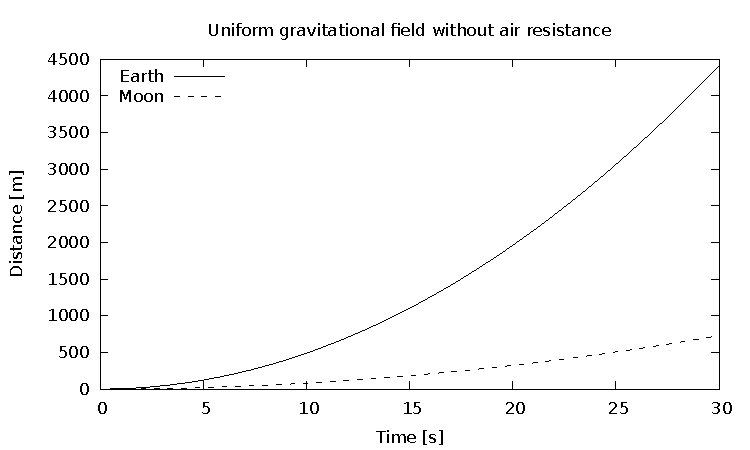
\includegraphics{gnuplot-bw}
% 	\caption{Cernobílá varianta obrázku generovaného programem Gnuplot}\label{fig:gnuplot-bw}
% \end{figure}
% 
% \begin{figure}\centering
% 	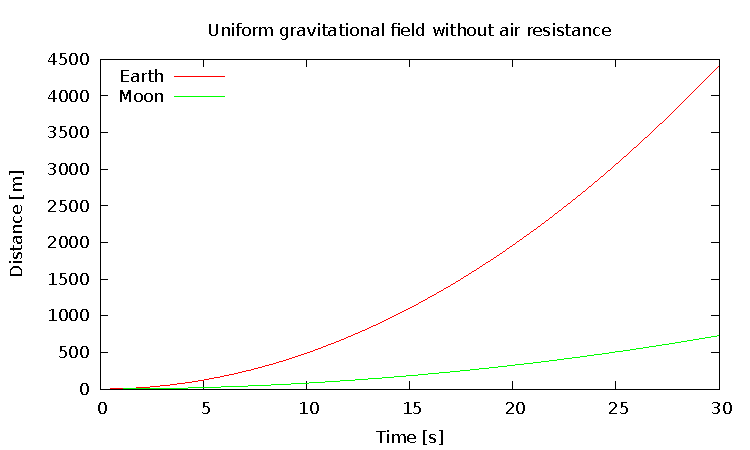
\includegraphics{gnuplot-col}
% 	\caption{Barevná varianta obrázku generovaného programem Gnuplot}\label{fig:gnuplot-col}
% \end{figure}
% 
% 
% \subsection{Tabulky}
% 
% Tabulky lze zadávat ruzne, napr. v~prostredí \verb|tabular|, avšak pro jejich vkládání platí to samé, co pro obrázky -- použijte plovoucí prostredí, v~tomto prípade \verb|table|. Napríklad tabulka \ref{tab:matematika} byla vložena tímto zpusobem.
% 
% \begin{table}\centering
% 	\caption[Príklad tabulky]{Zadávání matematiky}\label{tab:matematika}
% 	\begin{tabular}{|l|l|c|c|}\hline
% 		Typ		& Prostredí		& \LaTeX{}ovská zkratka	& \TeX{}ovská zkratka	\tabularnewline \hline \hline
% 		Text		& \verb|math|		& \verb|\(...\)|	& \verb|$...$|		\tabularnewline \hline
% 		Displayed	& \verb|displaymath|	& \verb|\[...\]|	& \verb|$$...$$|	\tabularnewline \hline
% 	\end{tabular}
% \end{table}
% 
% % % % % % % % % % % % % % % % % % % % % % % % % % % % 

\chapter{Obsah priloženého CD}

%upravte podle skutecnosti

\begin{figure}
	\dirtree{%
		.1 readme.txt\DTcomment{strucný popis obsahu CD}.
		.1 exe\DTcomment{adresár se spustitelnou formou implementace}.
		.1 src.
		.2 impl\DTcomment{zdrojové kódy implementace}.
		.2 thesis\DTcomment{zdrojová forma práce ve formátu \LaTeX{}}.
		.1 text\DTcomment{text práce}.
		.2 thesis.pdf\DTcomment{text práce ve formátu PDF}.
		.2 thesis.ps\DTcomment{text práce ve formátu PS}.
	}
\end{figure}

\end{document}